\chapter{Design} \label{chap:design}

\section{System Architecture}
  
\begin{figure}[ht]
\center
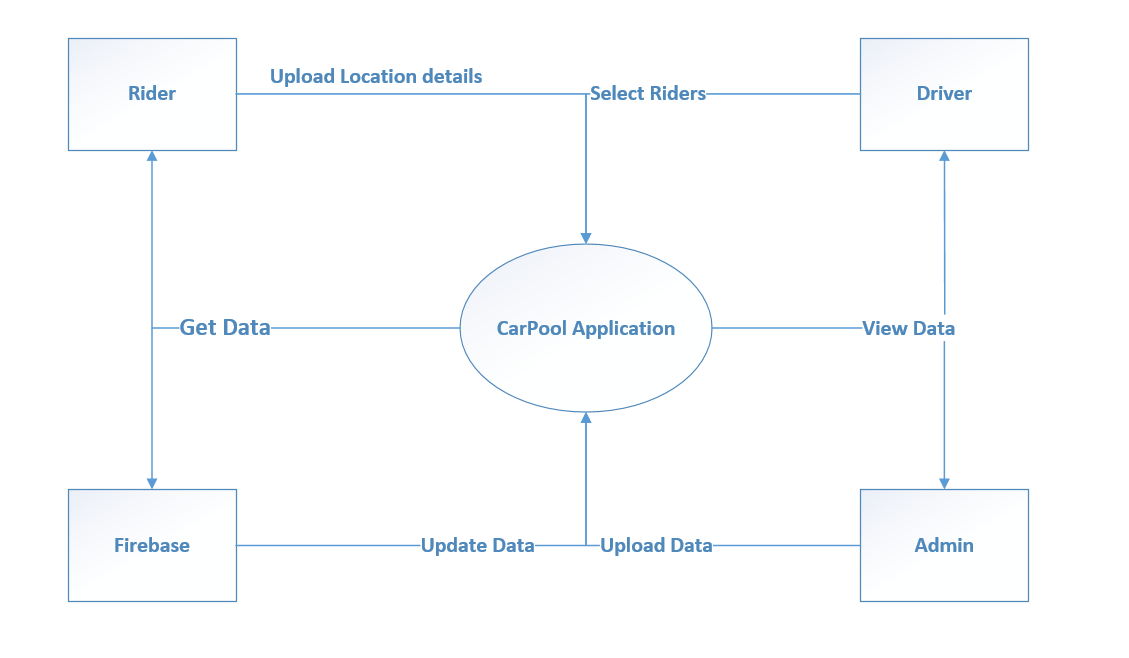
\includegraphics[width=1.0\textwidth]{SystemArchitecture}
\caption{Context Diagram}
\label{fig:Context Diagram}
\end{figure}
\begin{figure}[ht]
\center
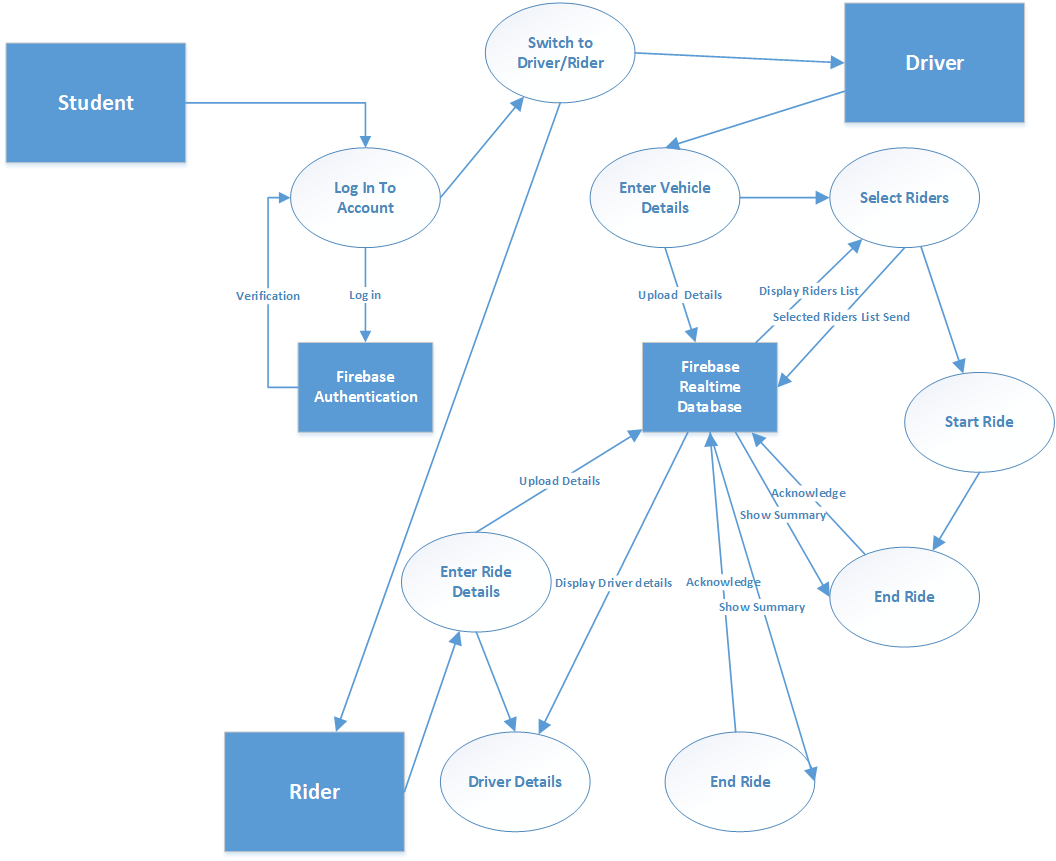
\includegraphics[width=1.1\textwidth]{SubSystem}
\caption{Sub System}
\label{fig:SubSystem}
\end{figure}

\section{Design Constraints} 
In our application, we added a list of pick up points for the ease of drivers. This is made easier when clients can select pick up points and drivers reach the destination without hassle. Due to the COVID-19 pandemic, we could not be supervised and guided properly. Hence this process was not added and executed.

\section{Design Methodology}
The design of a project is important for the structure of the application by using UML (Unified Modeling Language) which is a general purpose modelling language, that aims to define a standard way to visualize the way a system has been designed. It is quite similar to blueprints used in other fields of engineering. Reasons to use UML for project analysis and design are: 

\begin{itemize}
\item Complex applications needs collaboration and planning, hence require a transparent and concise way to communicate amongst them.
\item A lot of time is saved down the road when team is able to visualize the processes, user interactions and static structure of the system. These project designs will try to make the general idea of the project clearly understandable by identifying actors and functional / non-functional requirements, and also all the diagrams provide a transparent view about this project.
\end{itemize}

\section{High-Level Design}

\begin{figure}[!h]
\subsection{Package Diagram}
\center
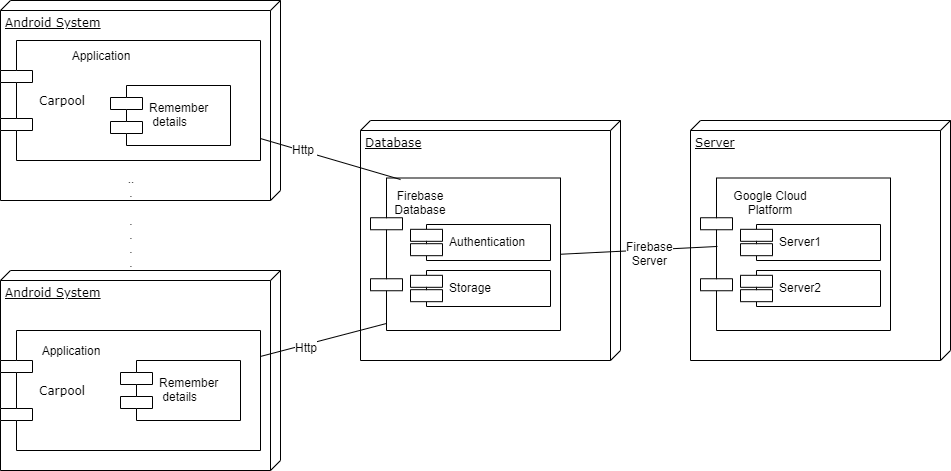
\includegraphics[width=1.0\textwidth]{PackageDiagram}
\caption{Package Diagram}
\label{fig:Package Diagram}
\end{figure}

\begin{figure}[!h]
\subsection{Interaction Diagram}
\center
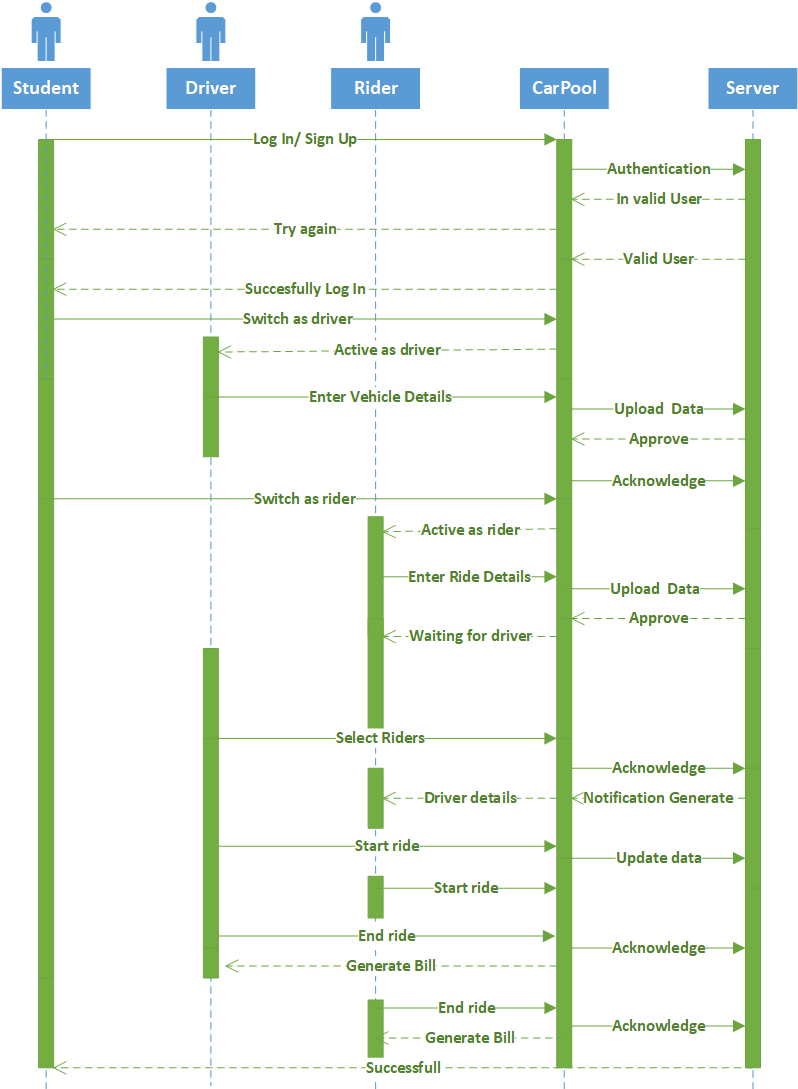
\includegraphics[width=15cm,height=25cm,keepaspectratio]{InteractionDiagram}
\caption{Process Interaction Diagram}
\label{fig:Process Interaction Diagram}
\end{figure}

\begin{figure}[!h]
\subsection{Deployment Diagram}
\center
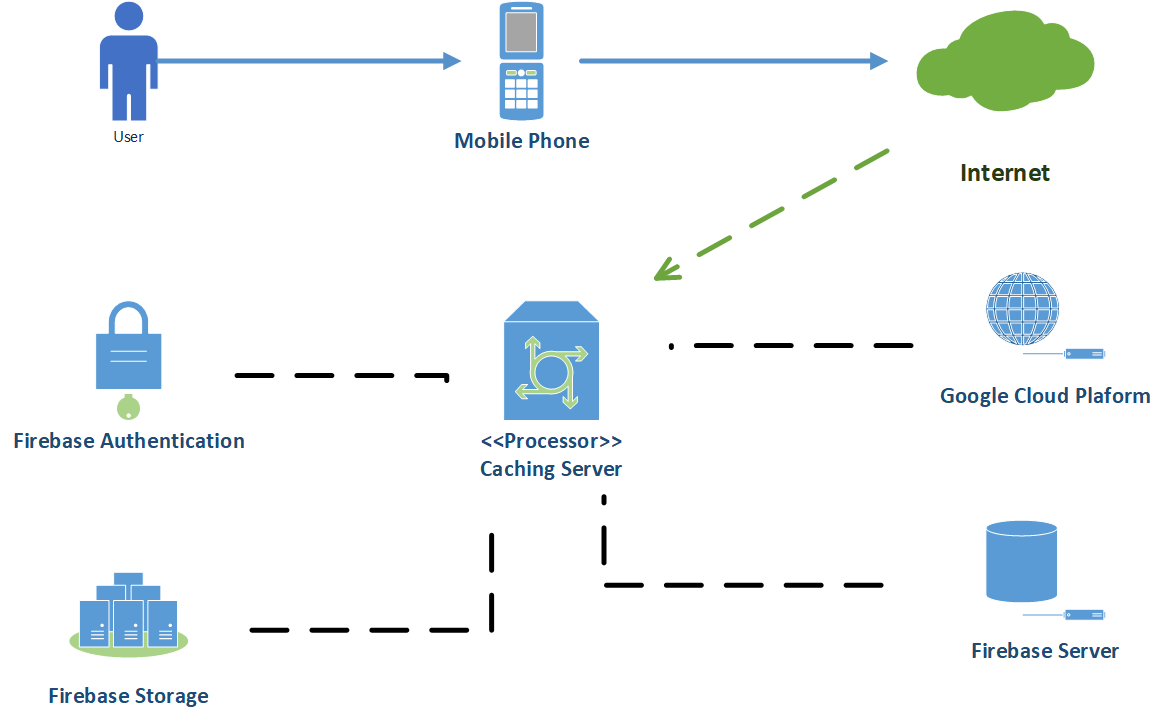
\includegraphics[width=15cm,height=20cm,keepaspectratio]{DeploymentDiagram}
\caption{Deployment Diagram}
\label{fig:Deployment Diagram}
\end{figure}

\clearpage

\subsection{Modules}

The application is divided into three modules:
\begin{itemize}
\item User Registration
\item Driver
\item Rider
\end{itemize}

\subsubsection{User Registration}
In this module, the user must enter his/her credentials to use this application. Users should be student and currently enrolled in Air University. The user should enter the details first: name, last Name, student email, university registration id, contact no, password. So user using these registration details will be able to use application. This authentication process is used to avoid malpractice as this module is there to verify student details.


\subsubsection{Driver}
In this module, the user acts as a driver. This module consists of 8 activities which contains 2 fragments (map, passenger list). The driver can use the map fragment to see the passenger pickup points and current location and can use passenger list fragment to see the list of passengers. Driver module also contains the activities to enter vehicle details and see summary of the ride.

\subsubsection{Rider}
In this module, the user acts as a rider. This module consists of 4 activities which contains 2 fragments (map, driver details). The passenger can use the map fragment to see the pickup point and current location and can use driver detail fragment to see the detail of driver. Rider module also contains the activities to enter trip detail and see summary of the ride.

\subsection{Security} 		
This application does not disclose any personal information of any user and does not collect any sensitive information from it's own users.

\section{Low Level Design}
\begin{figure}[!h]
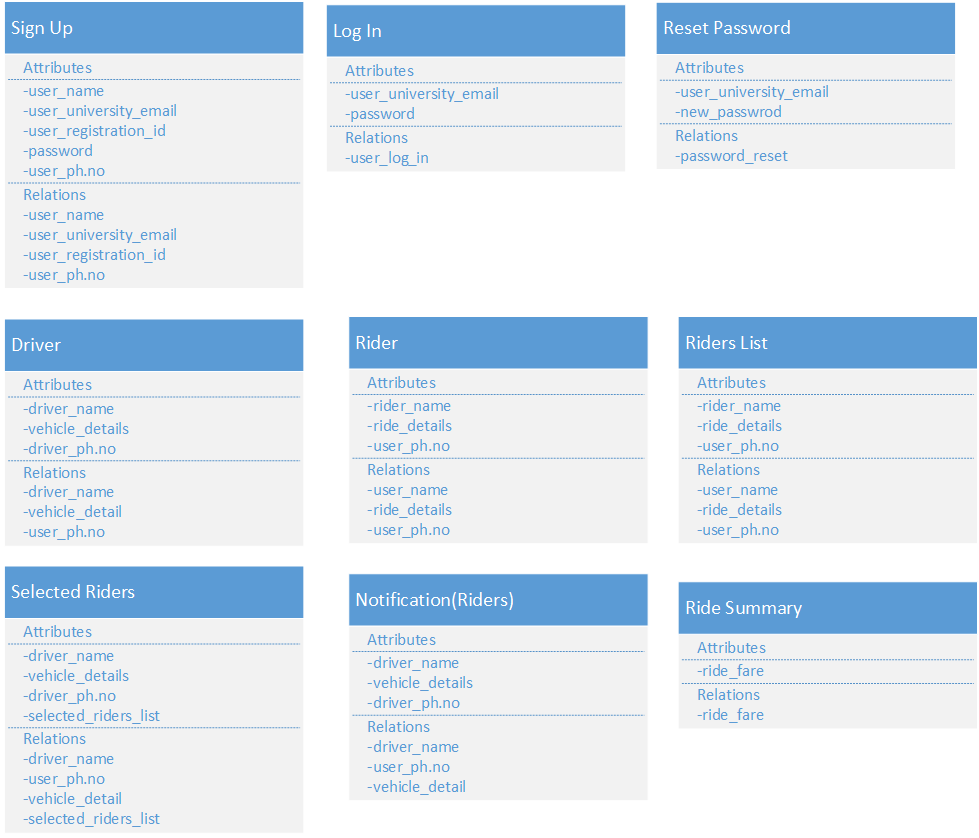
\includegraphics[width=16cm,height=25cm,keepaspectratio]{LowLevelDesign}
\caption{Low Level Design}
\label{fig:Low Level Design}
\end{figure} 

\subsection{Database Design}
Firebase platform provides a cloud-hosted real time database. It is a NoSQL cloud database. Data synchronizes among all clients and stays available even when the app goes offline. As it is a NoSQL database, so its functionality is different as compared to a relational database. The data is stored in the form of collections and documents. There is no relationship between classes, so there won’t be any schema of our database. Data gets stored as JSON Objects. it is more like a cloud-hosted JSON tree. When a person adds data to the JSON tree, it becomes a node in the existing JSON structure with an associated key. The best method is to use the denormalization technique; using which we split data into separate paths. It becomes easier to download the data in separate calls as required.

\subsection{GUI Design}
Our application contains more than fifteen screens. Different screens based on user type are:

\begin{figure}
\subsubsection{Welcome Interface}
This is the interface that shows up to the user when he opens the application. This interface is composed of the application’s name, a logo and a slang which describe the application alongside a "Get Started" button which directs the user to login screen.

\centering
\subfloat[Welcome Screen]{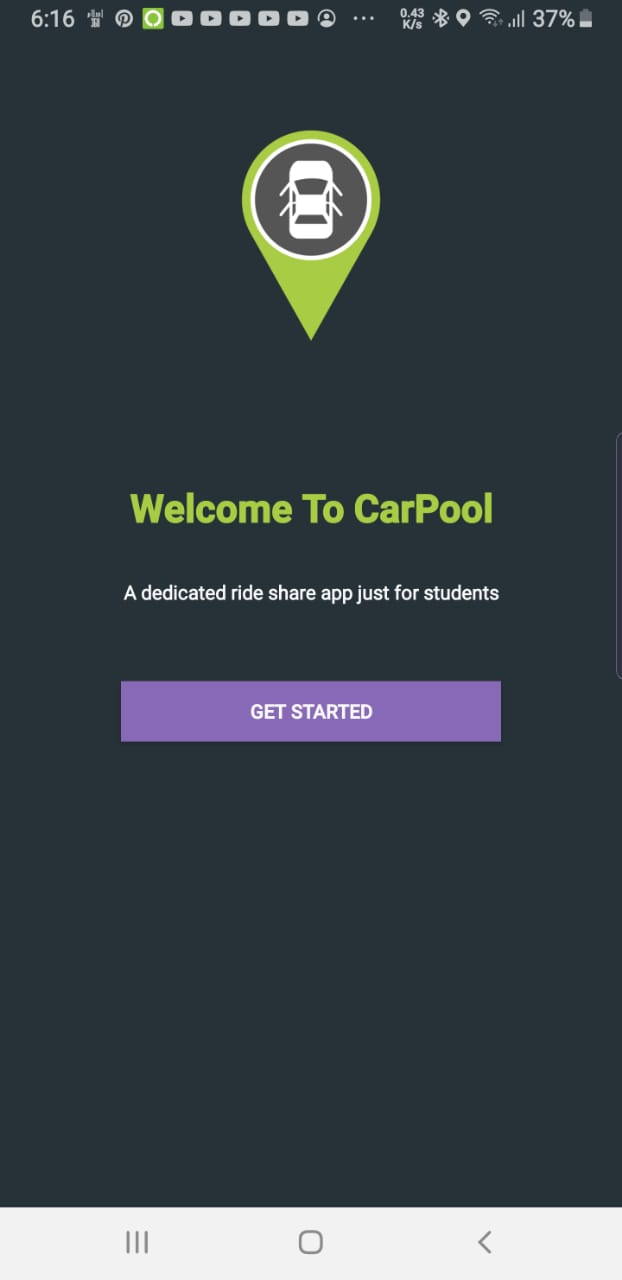
\includegraphics[width = 2in]{S1}}
\end{figure}

\begin{figure}
\subsubsection{Authentication Interfaces}
The authentication interface is made as simple as possible while also being very pretty and professional. It utilizes Firebase auth as a backend which allows for a secure connection to the database plus encrypted passwords for extra security. This interface also contains options to recover password in case the user has forgotten their password.

\centering
\hspace*{\fill}
\subfloat[Login Screen]{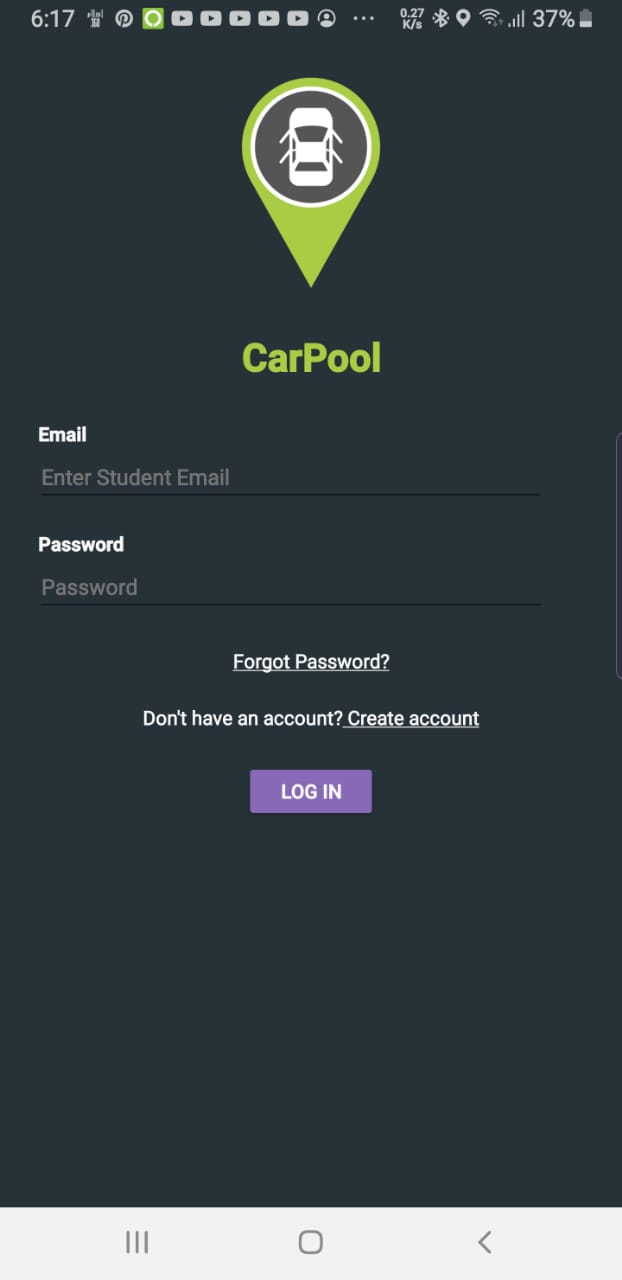
\includegraphics[height=3.5in, width = 2in]{S2}}\hfill 
\subfloat[Signup Screen]{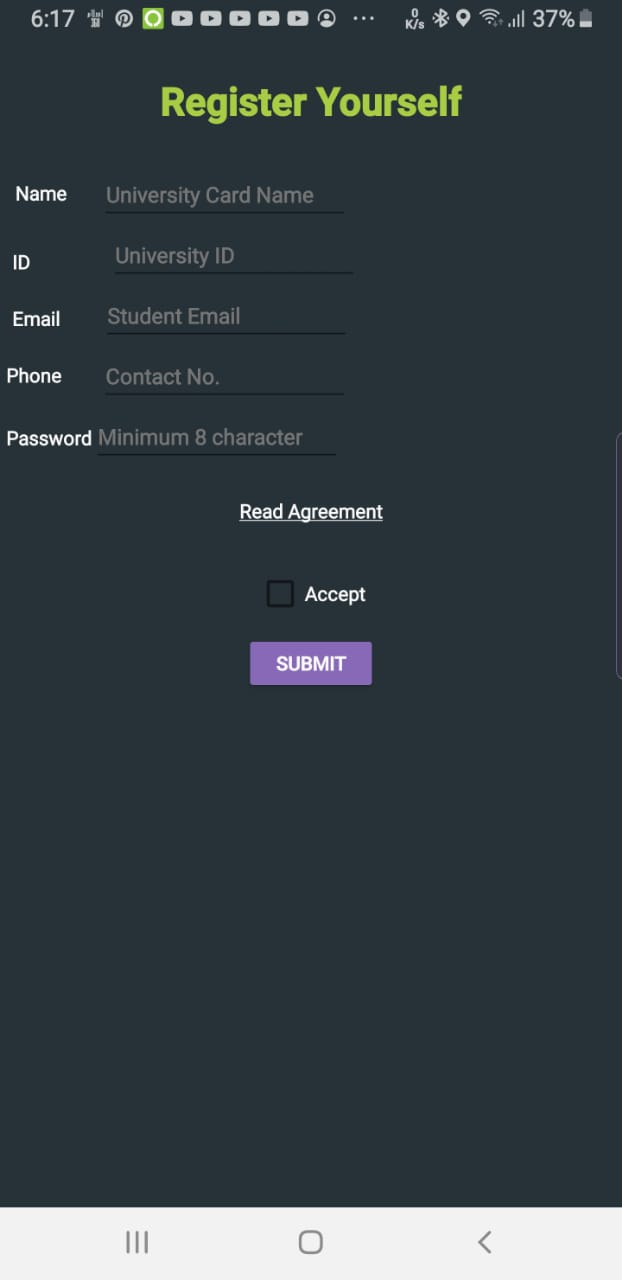
\includegraphics[height=3.5in, width = 2in]{S3}}\hfil
\subfloat[Forgot Password Screen]{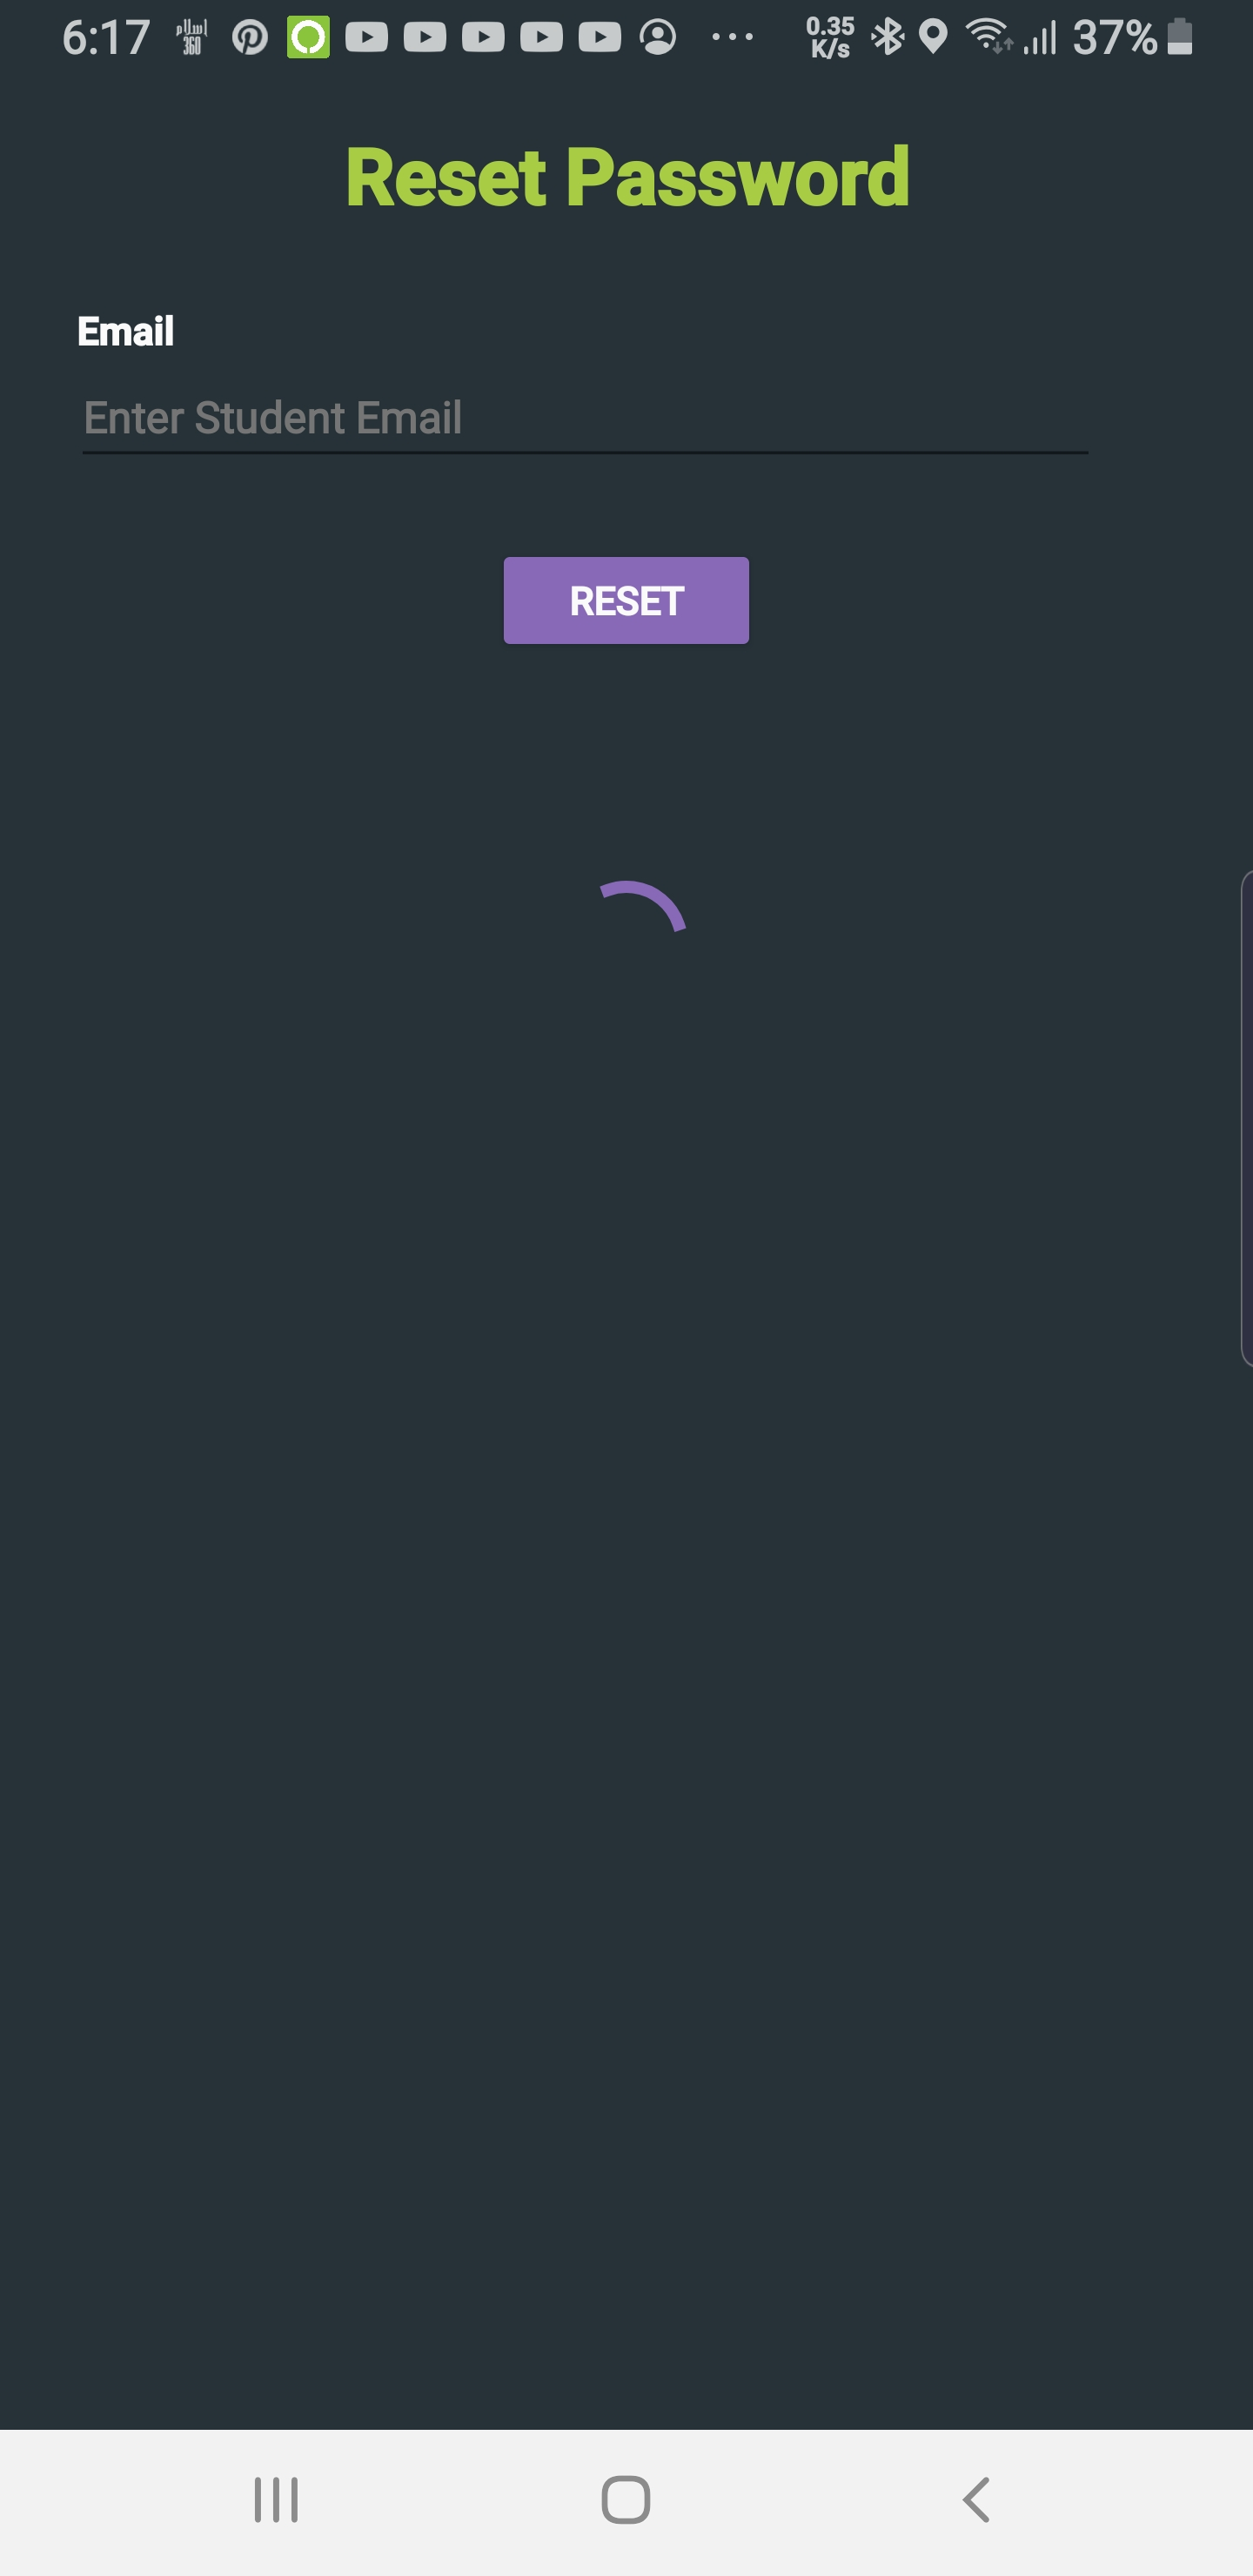
\includegraphics[height=3.5in, width = 2in]{S4}}
\end{figure}

\begin{figure}
\subsubsection{Type Switching Interface}
This is the interface that shows up to the user when he’s logged in into the application. This interface is composed of the application’s name and a logo alongside a switch button, which lets the user select his/her user type.

\centering
\subfloat[Select User Type Screen]{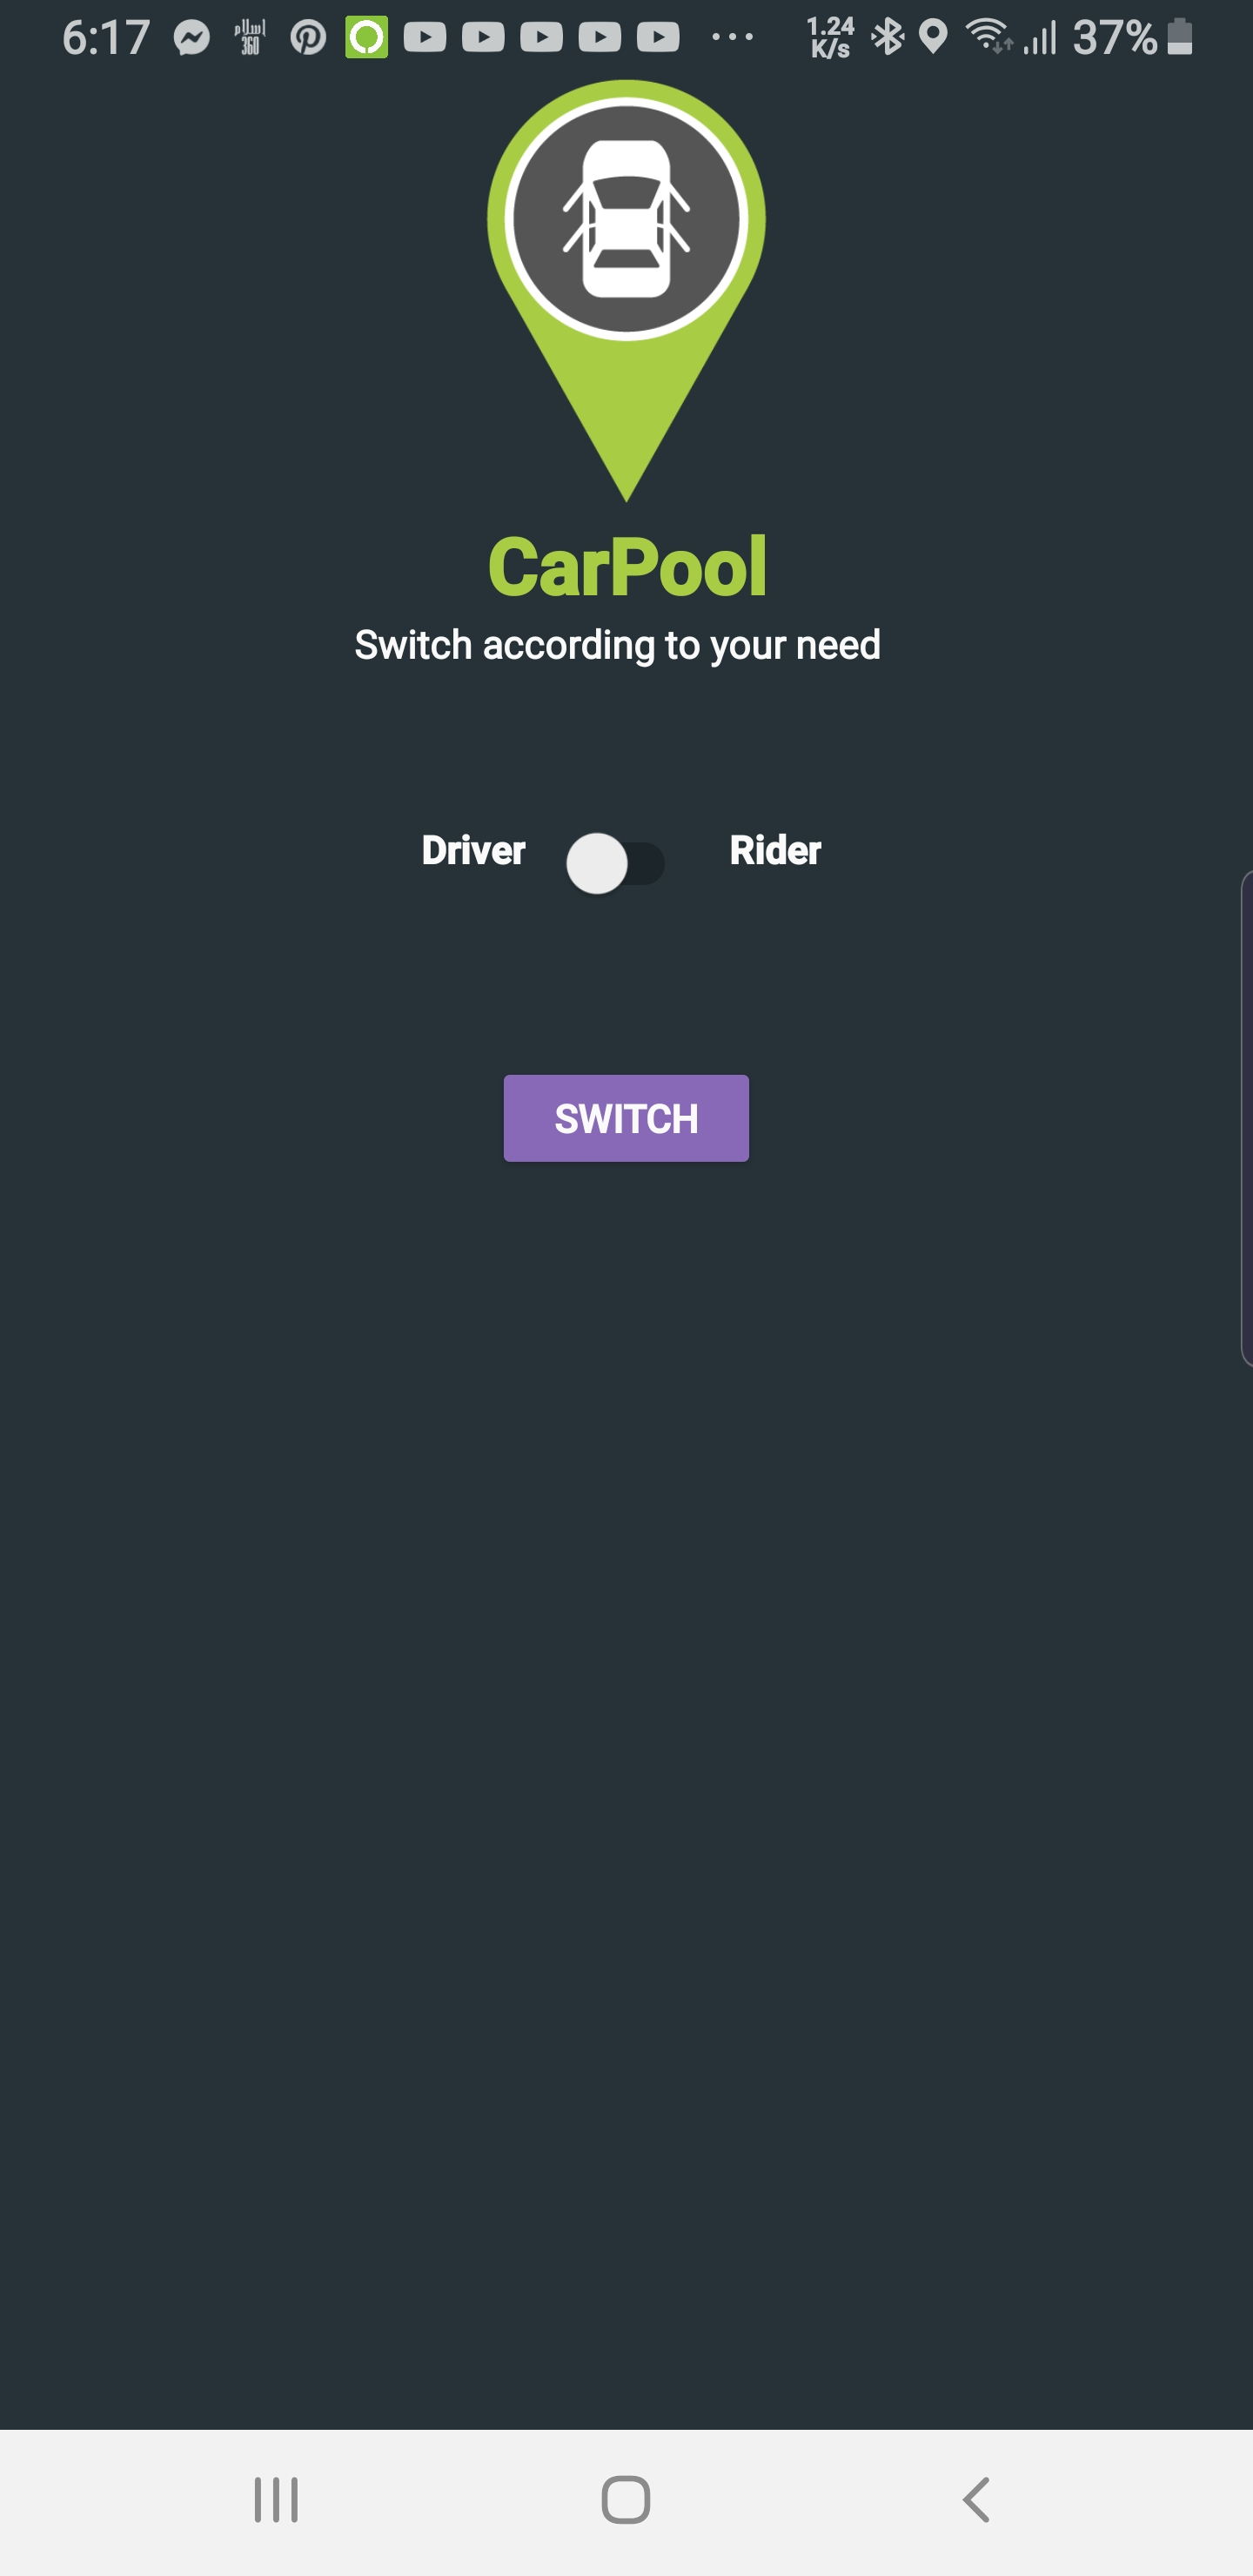
\includegraphics[width = 2in]{S5}}
\end{figure}

\begin{figure} 
\subsubsection{Rider Interfaces}
These interfaces are used by the passengers to post ride details for drivers to see and select riders. These interfaces are extremely customizable and professional and are created by using Google Places API, Google Direction API, Google Map API. We have created a very organized and efficient algorithm to optimize the results when passengers search for a driver. When rider picks an origin and a destination using Places AutoComplete API, the algorithm uses a combination of Geolocation and Places API to find the full address, city and sub city.

\hspace*{\fill}
\subfloat[Enter Ride Detail Screen]{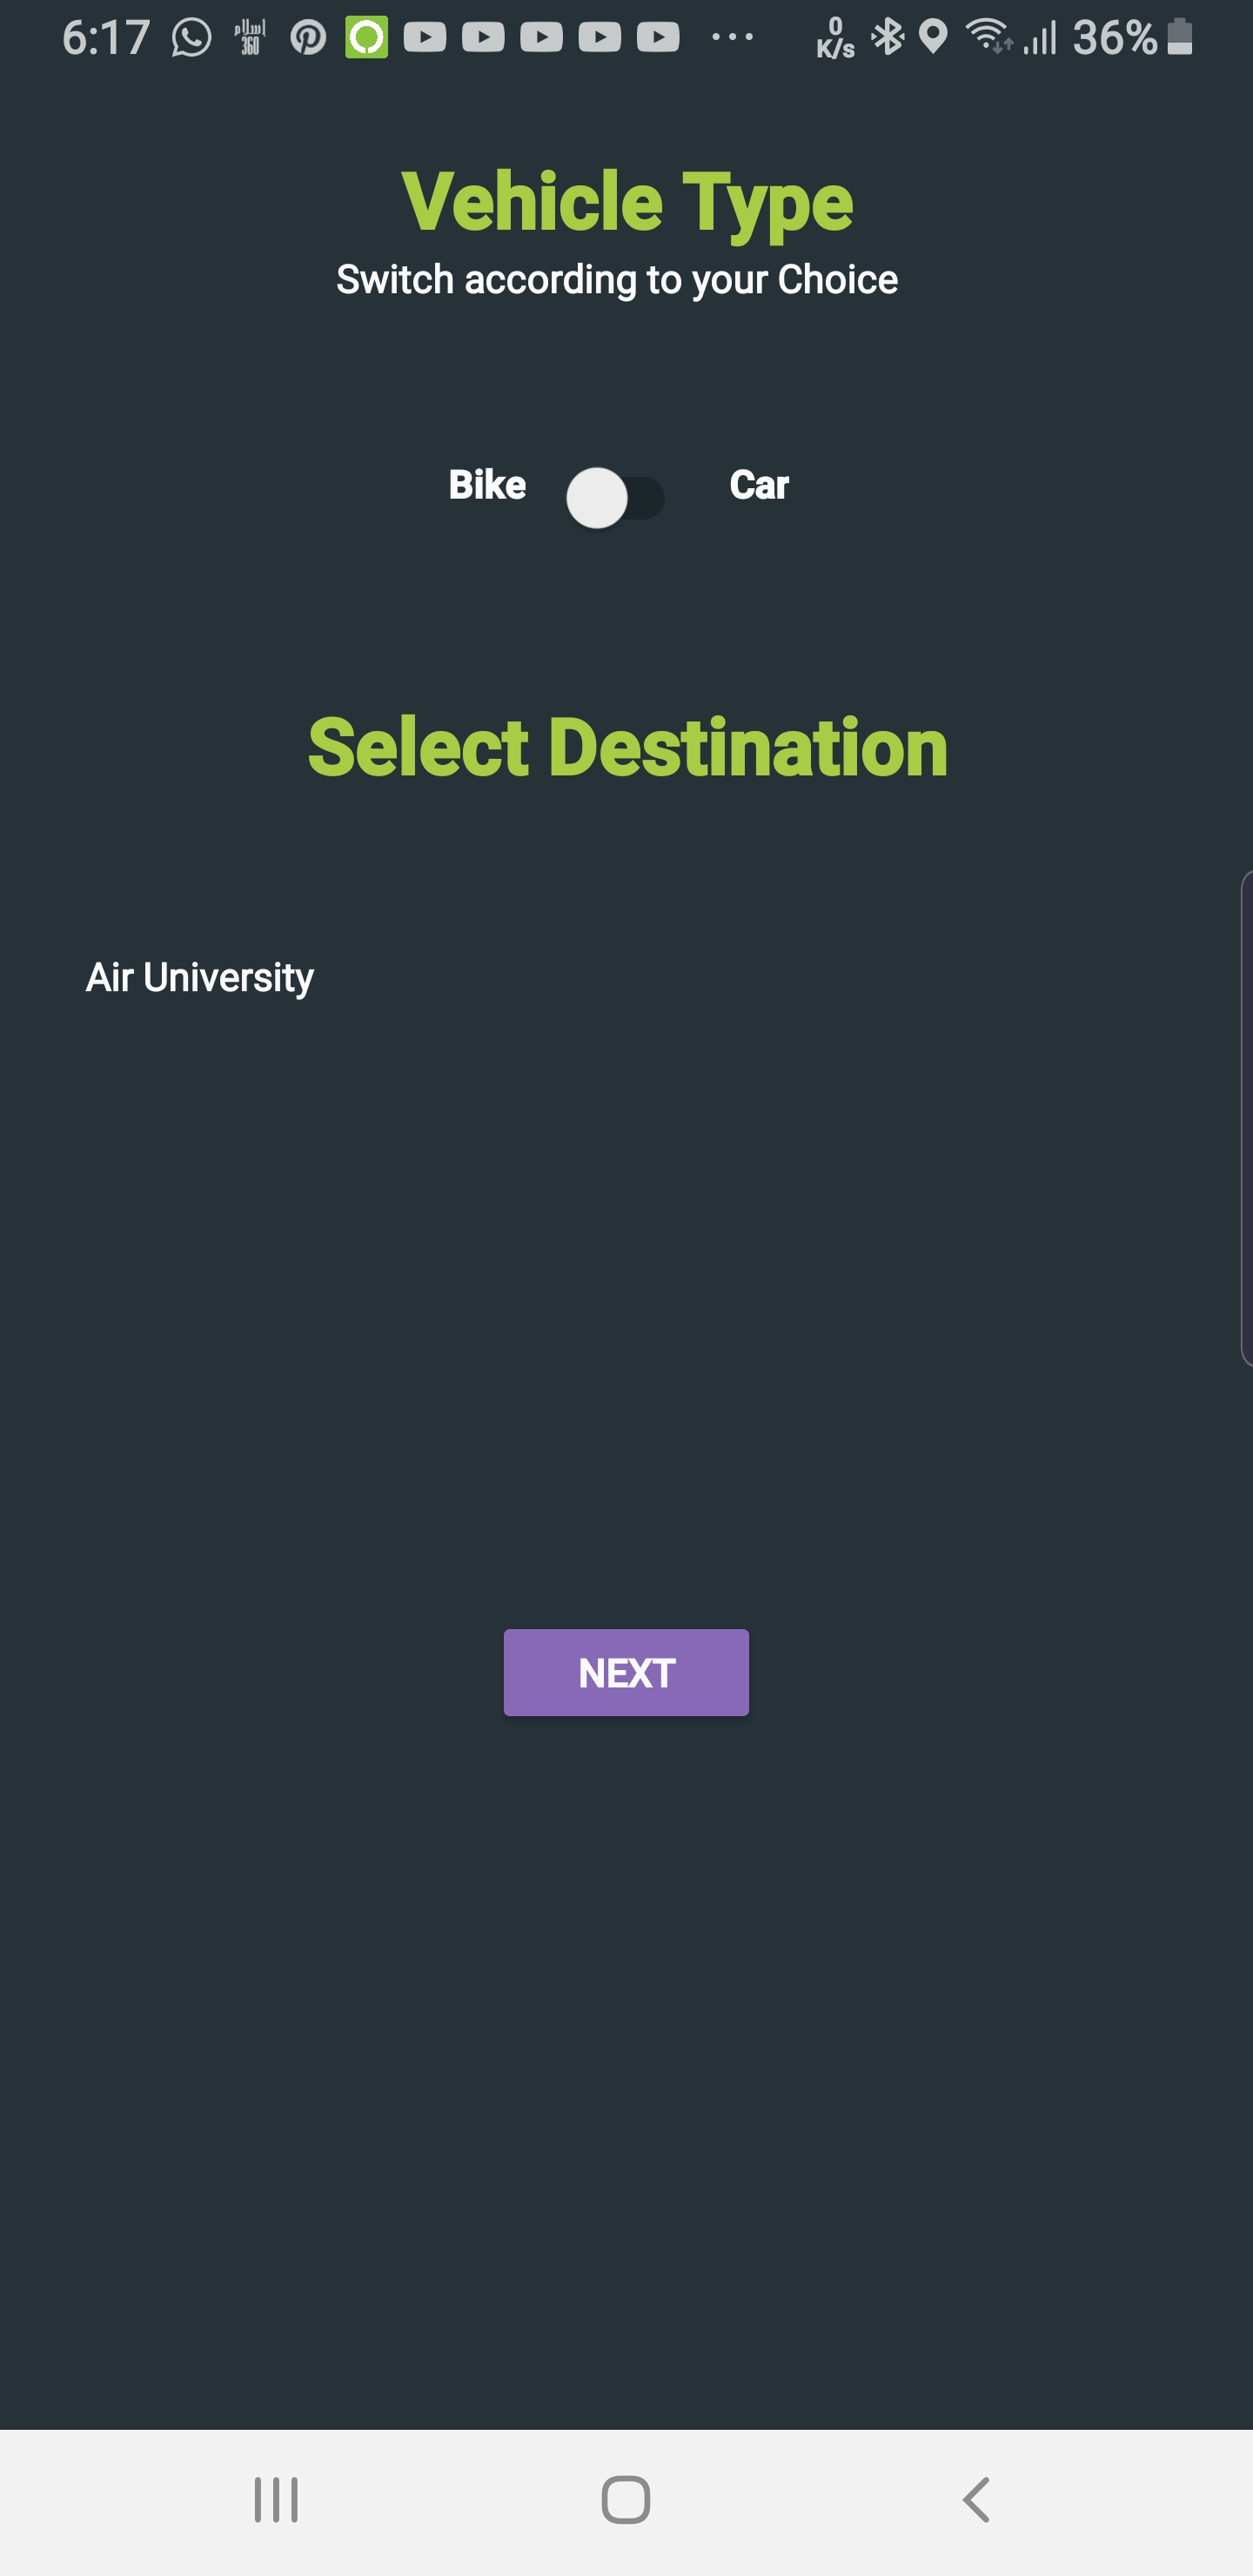
\includegraphics[height = 3.5in, width = 2in]{S6}}\hfill 
\subfloat[Map Screen]{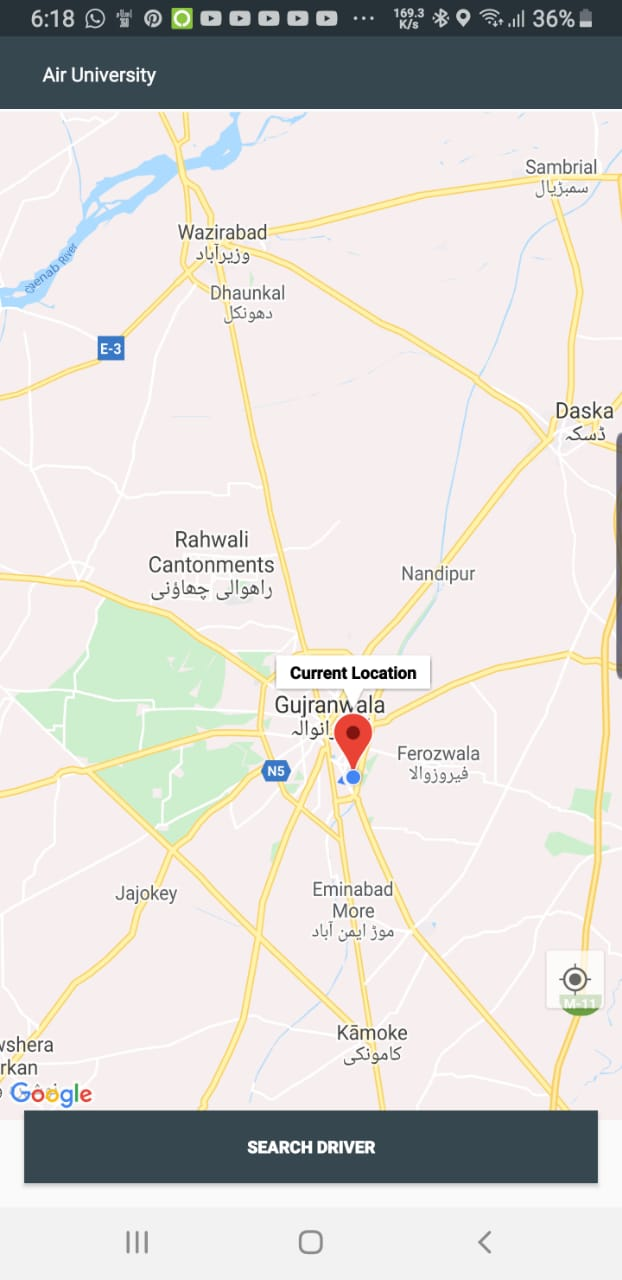
\includegraphics[height = 3.5in, width = 2in]{S7}}\\
\hspace*{\fill}
\subfloat[Driver Detail Screen]{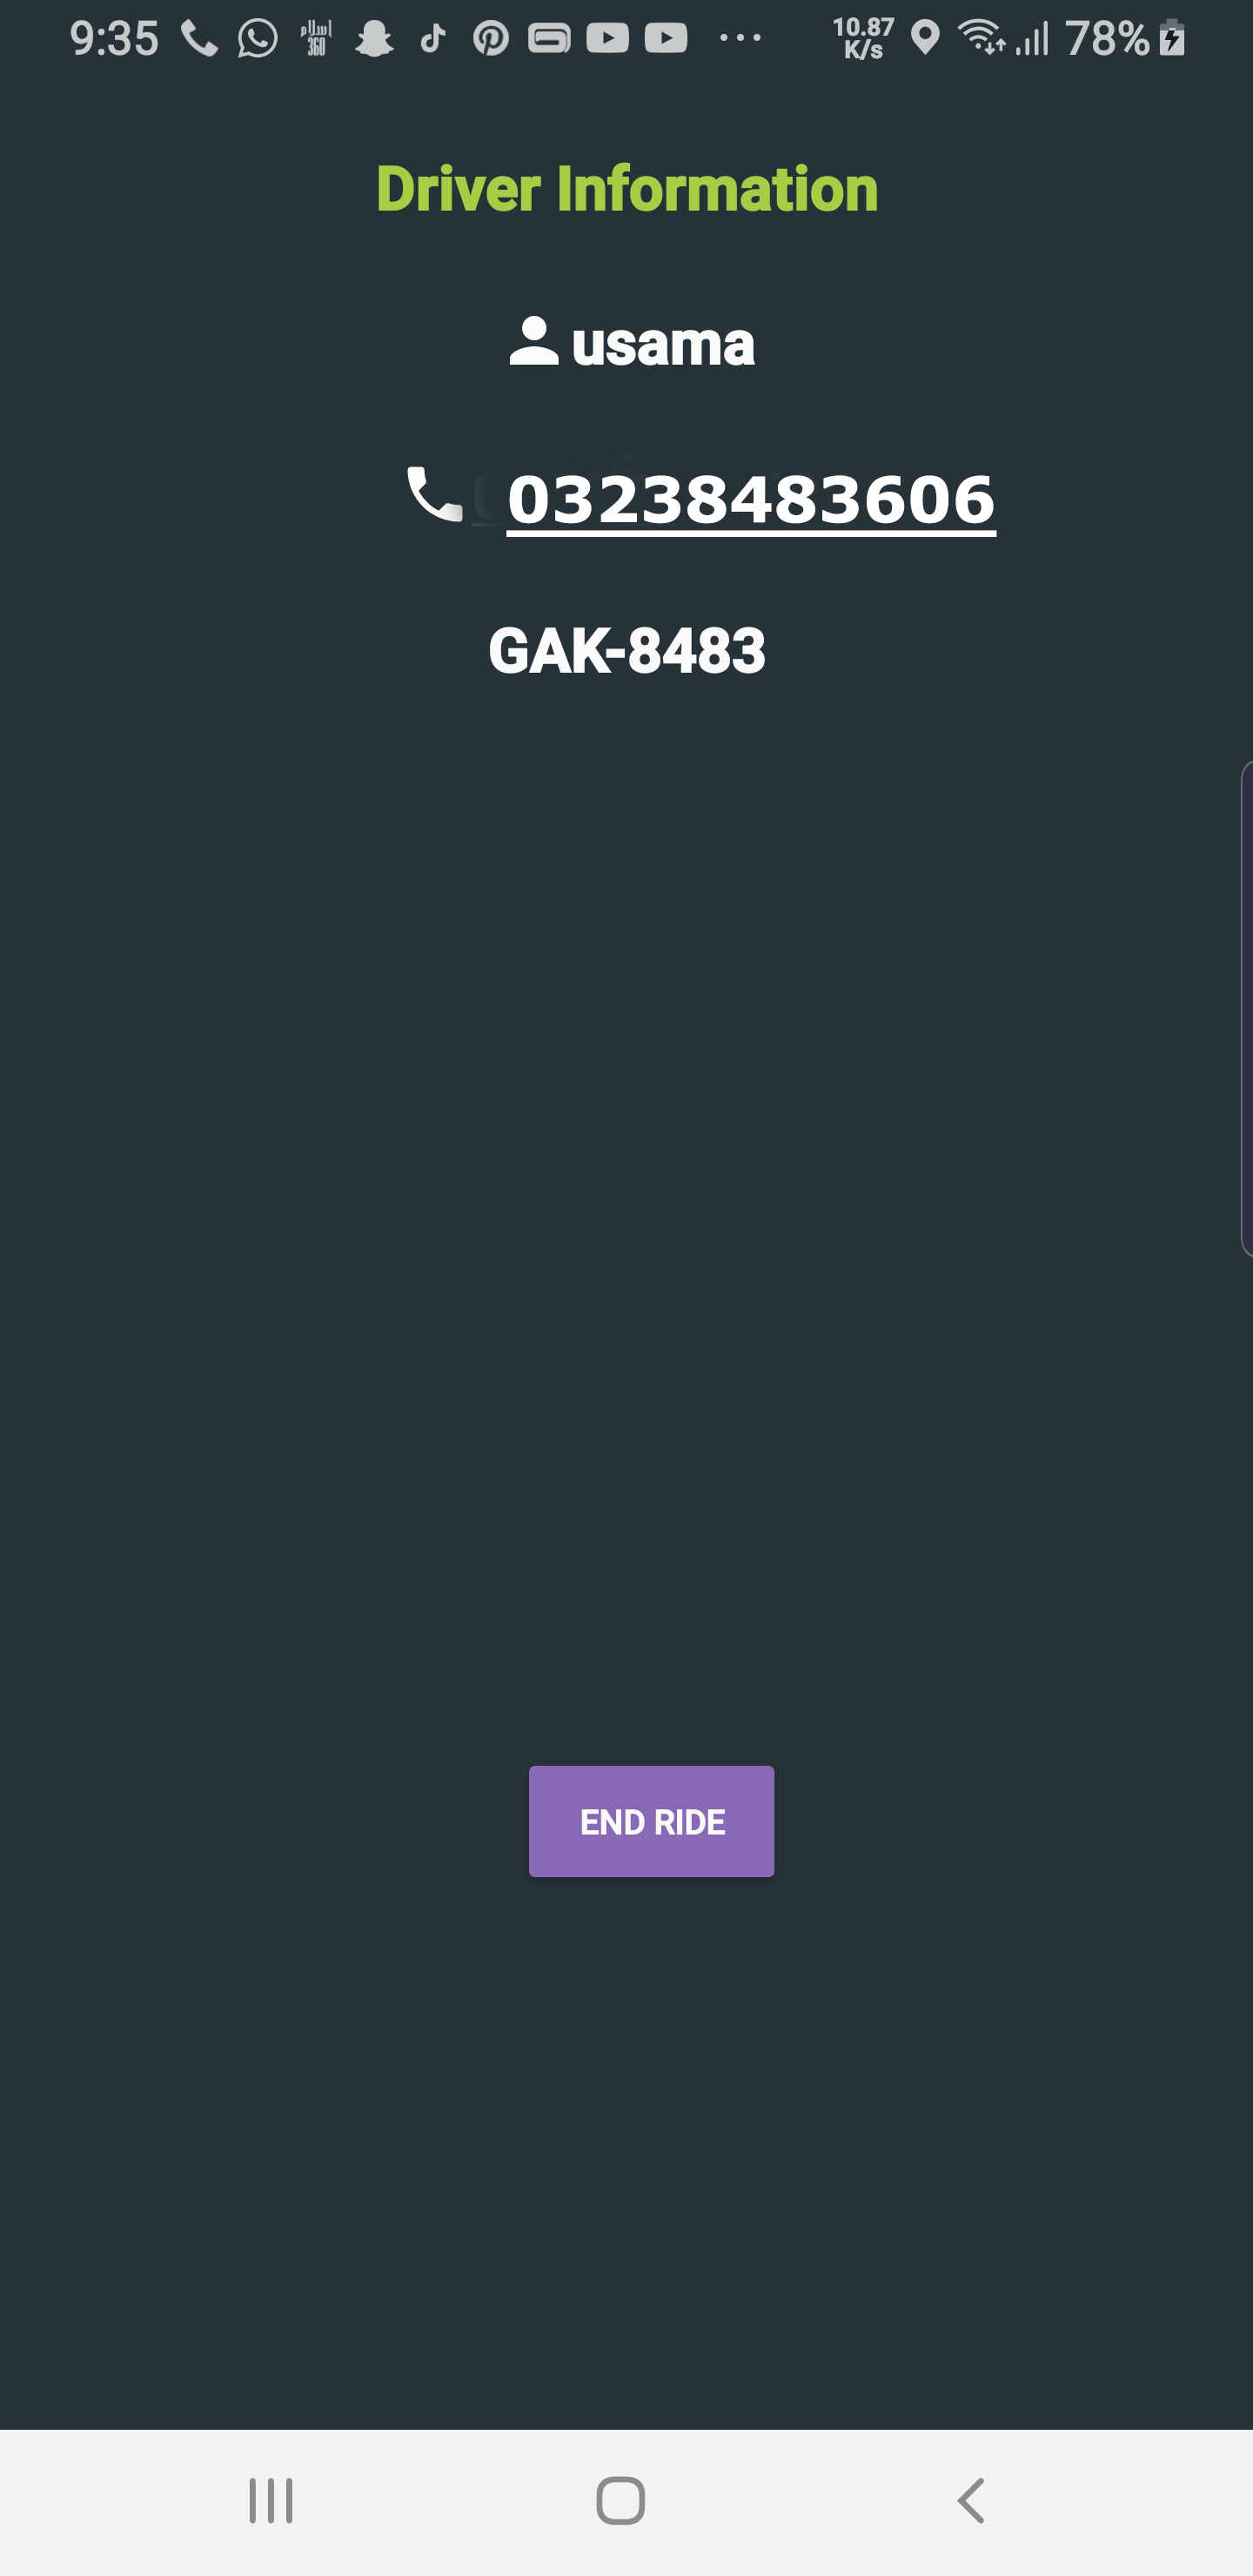
\includegraphics[height = 3.5in, width = 2in]{S8}}\hfill 
\subfloat[Ride Summary Screen]{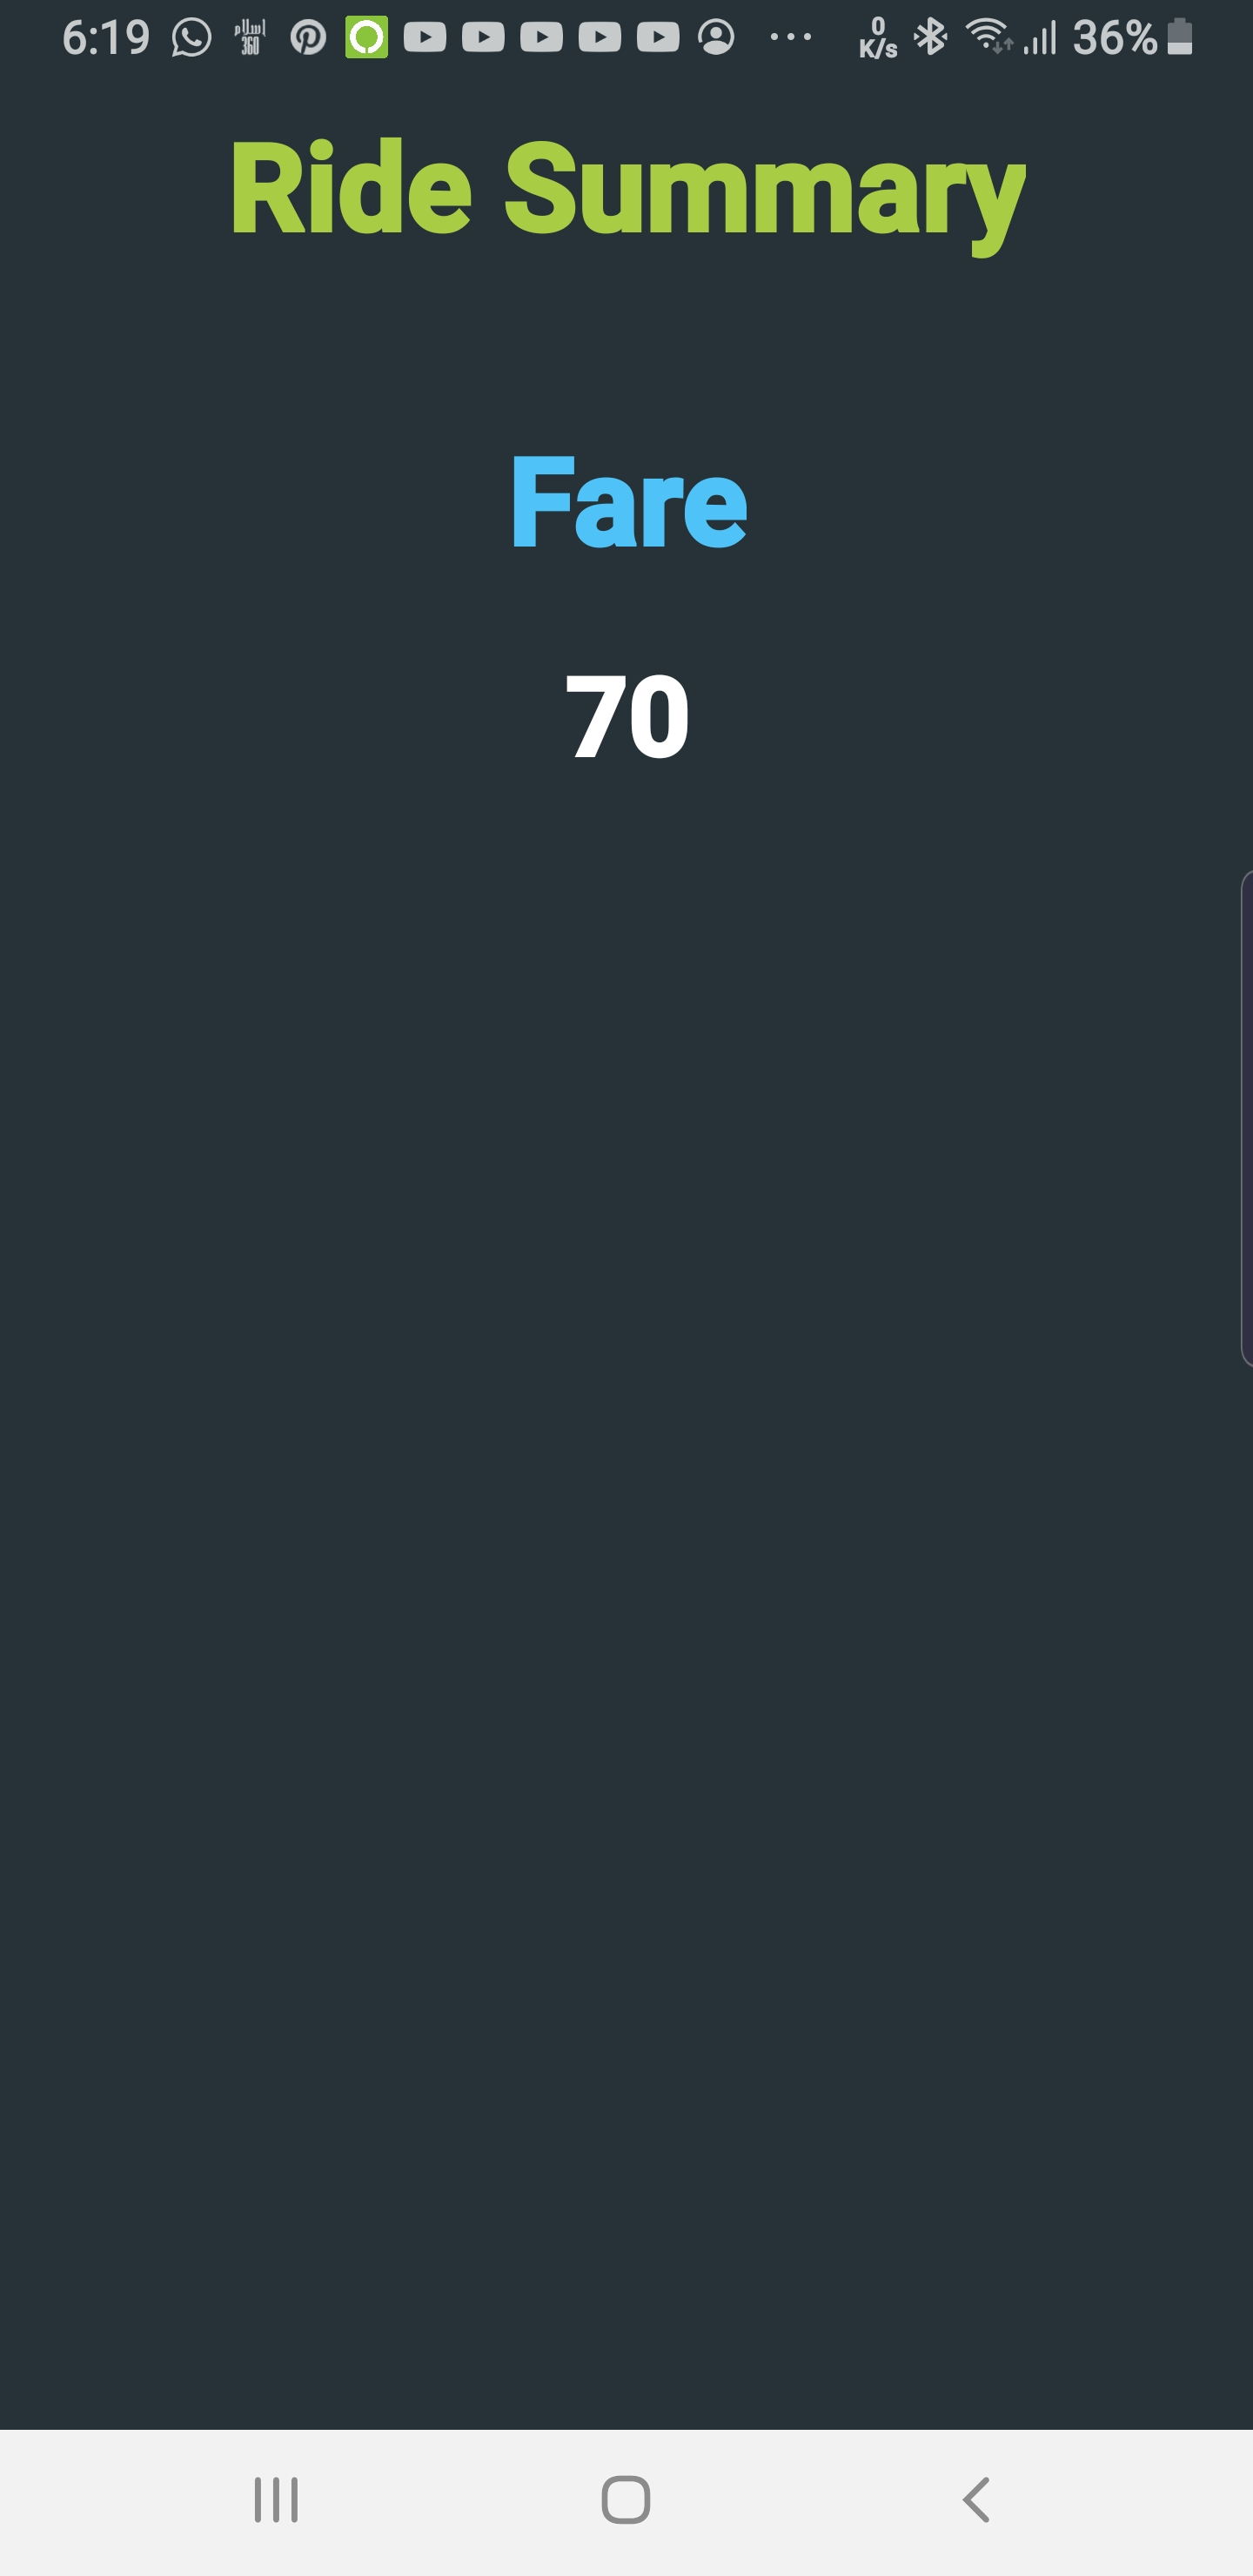
\includegraphics[height = 3.5in, width = 2in]{S9}}
\hspace*{\fill}
\end{figure}

\begin{figure}
\subsubsection{Driver Interfaces}
These interfaces are used by rider to enter vehicle detail, and see and select the passengers for trip. These form are extremely customizable and professional and are created by using Google Places API. In this interface, we have created a very organized and efficient algorithm to optimize the results.

\hspace*{\fill}
\subfloat[Enter Vehicle Detail Screen]{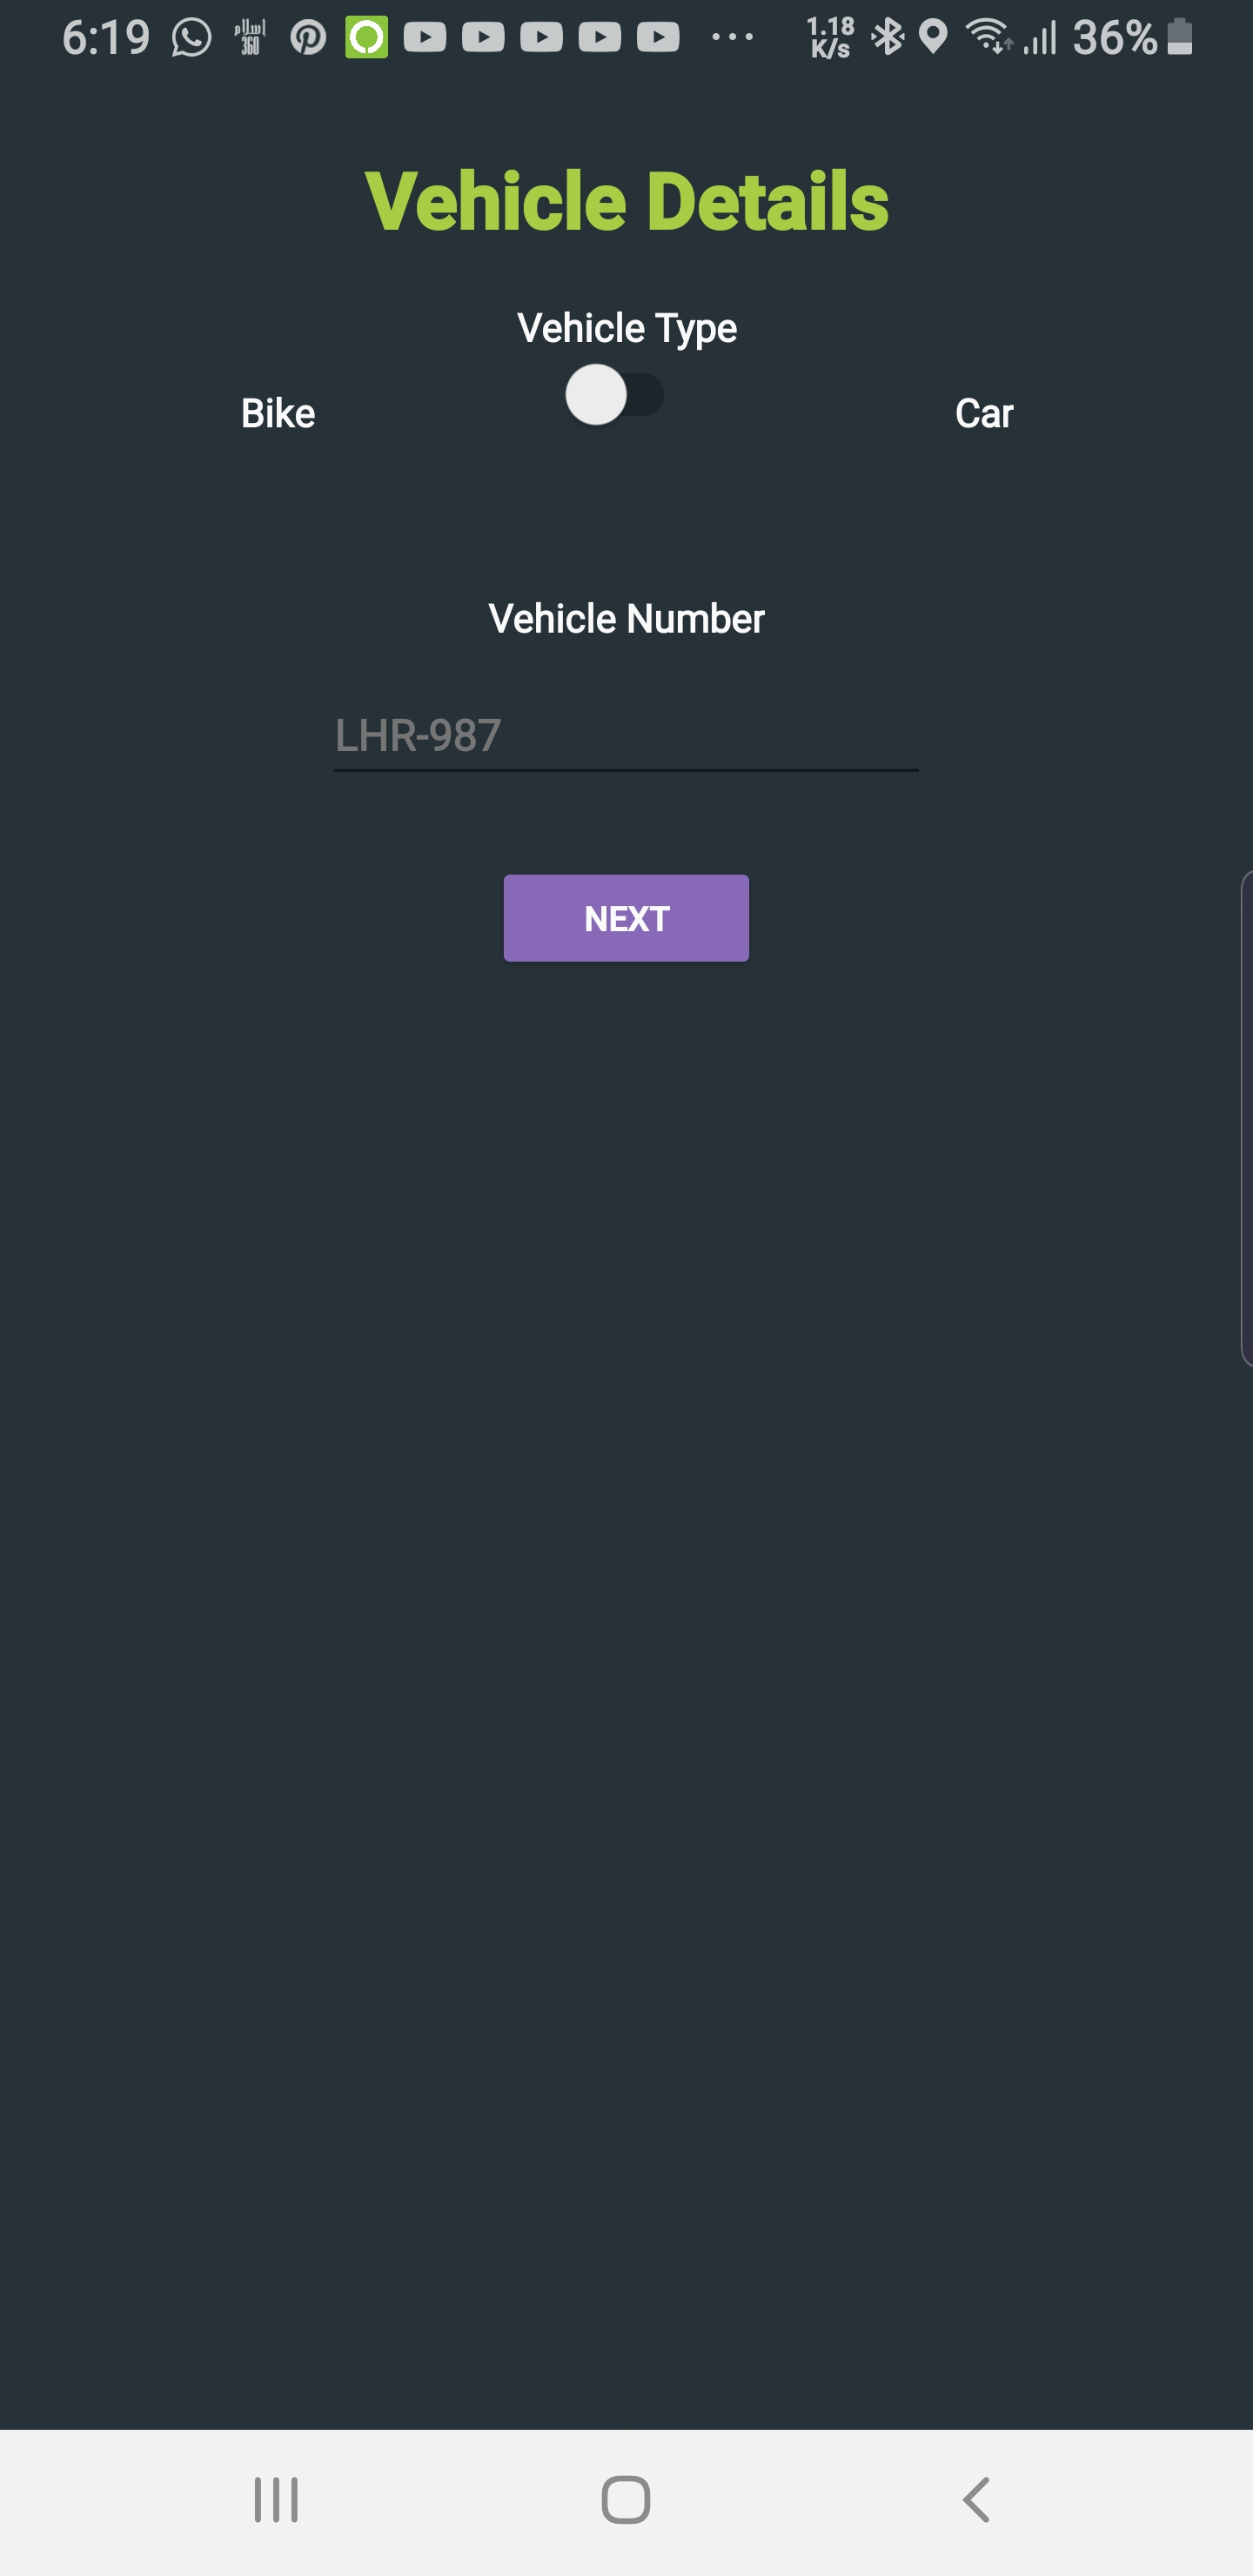
\includegraphics[width = 2in]{S10}}\hfill 
\subfloat[Driver Map Screen]{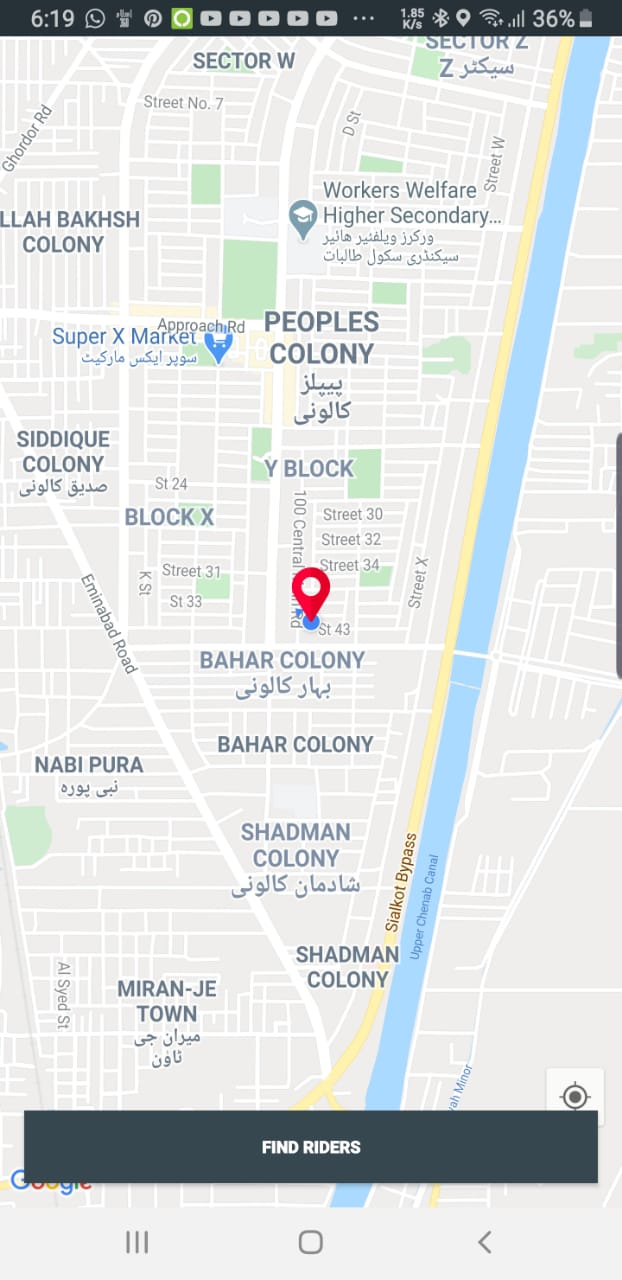
\includegraphics[width = 2in]{S11}}
\hspace*{\fill}

The algorithm uses a combination of Geolocation and Places API to find the full address, city and sub city.

\end{figure}

\begin{figure}
\hspace*{\fill}
\subfloat[Selected Passengers Screen]{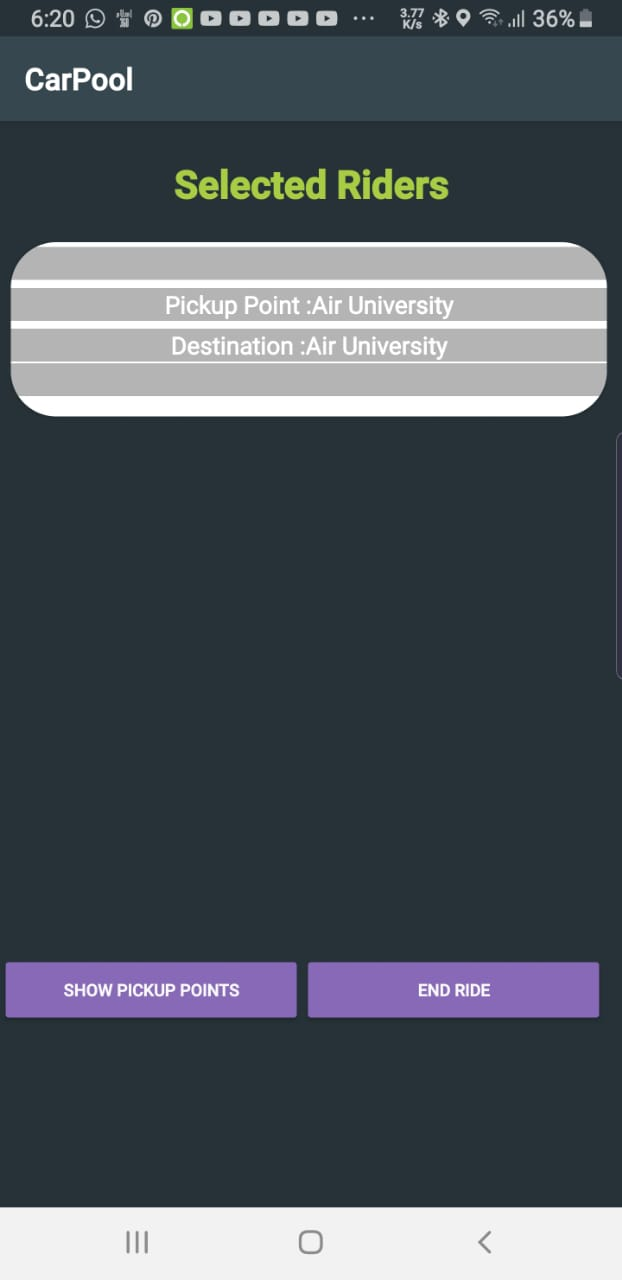
\includegraphics[width = 2in]{S14}}\hfill 
\subfloat[Passengers Pickup Points Screen]{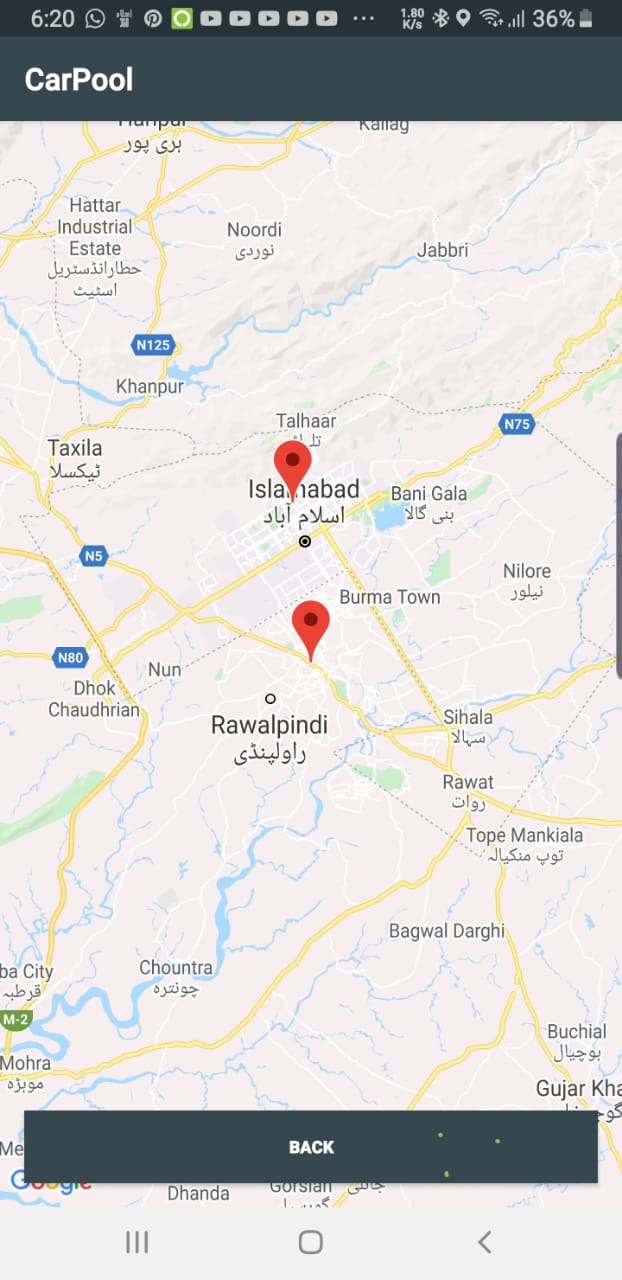
\includegraphics[width = 2in]{S15}}\\
\hspace*{\fill}
\subfloat[Rider List Screen]{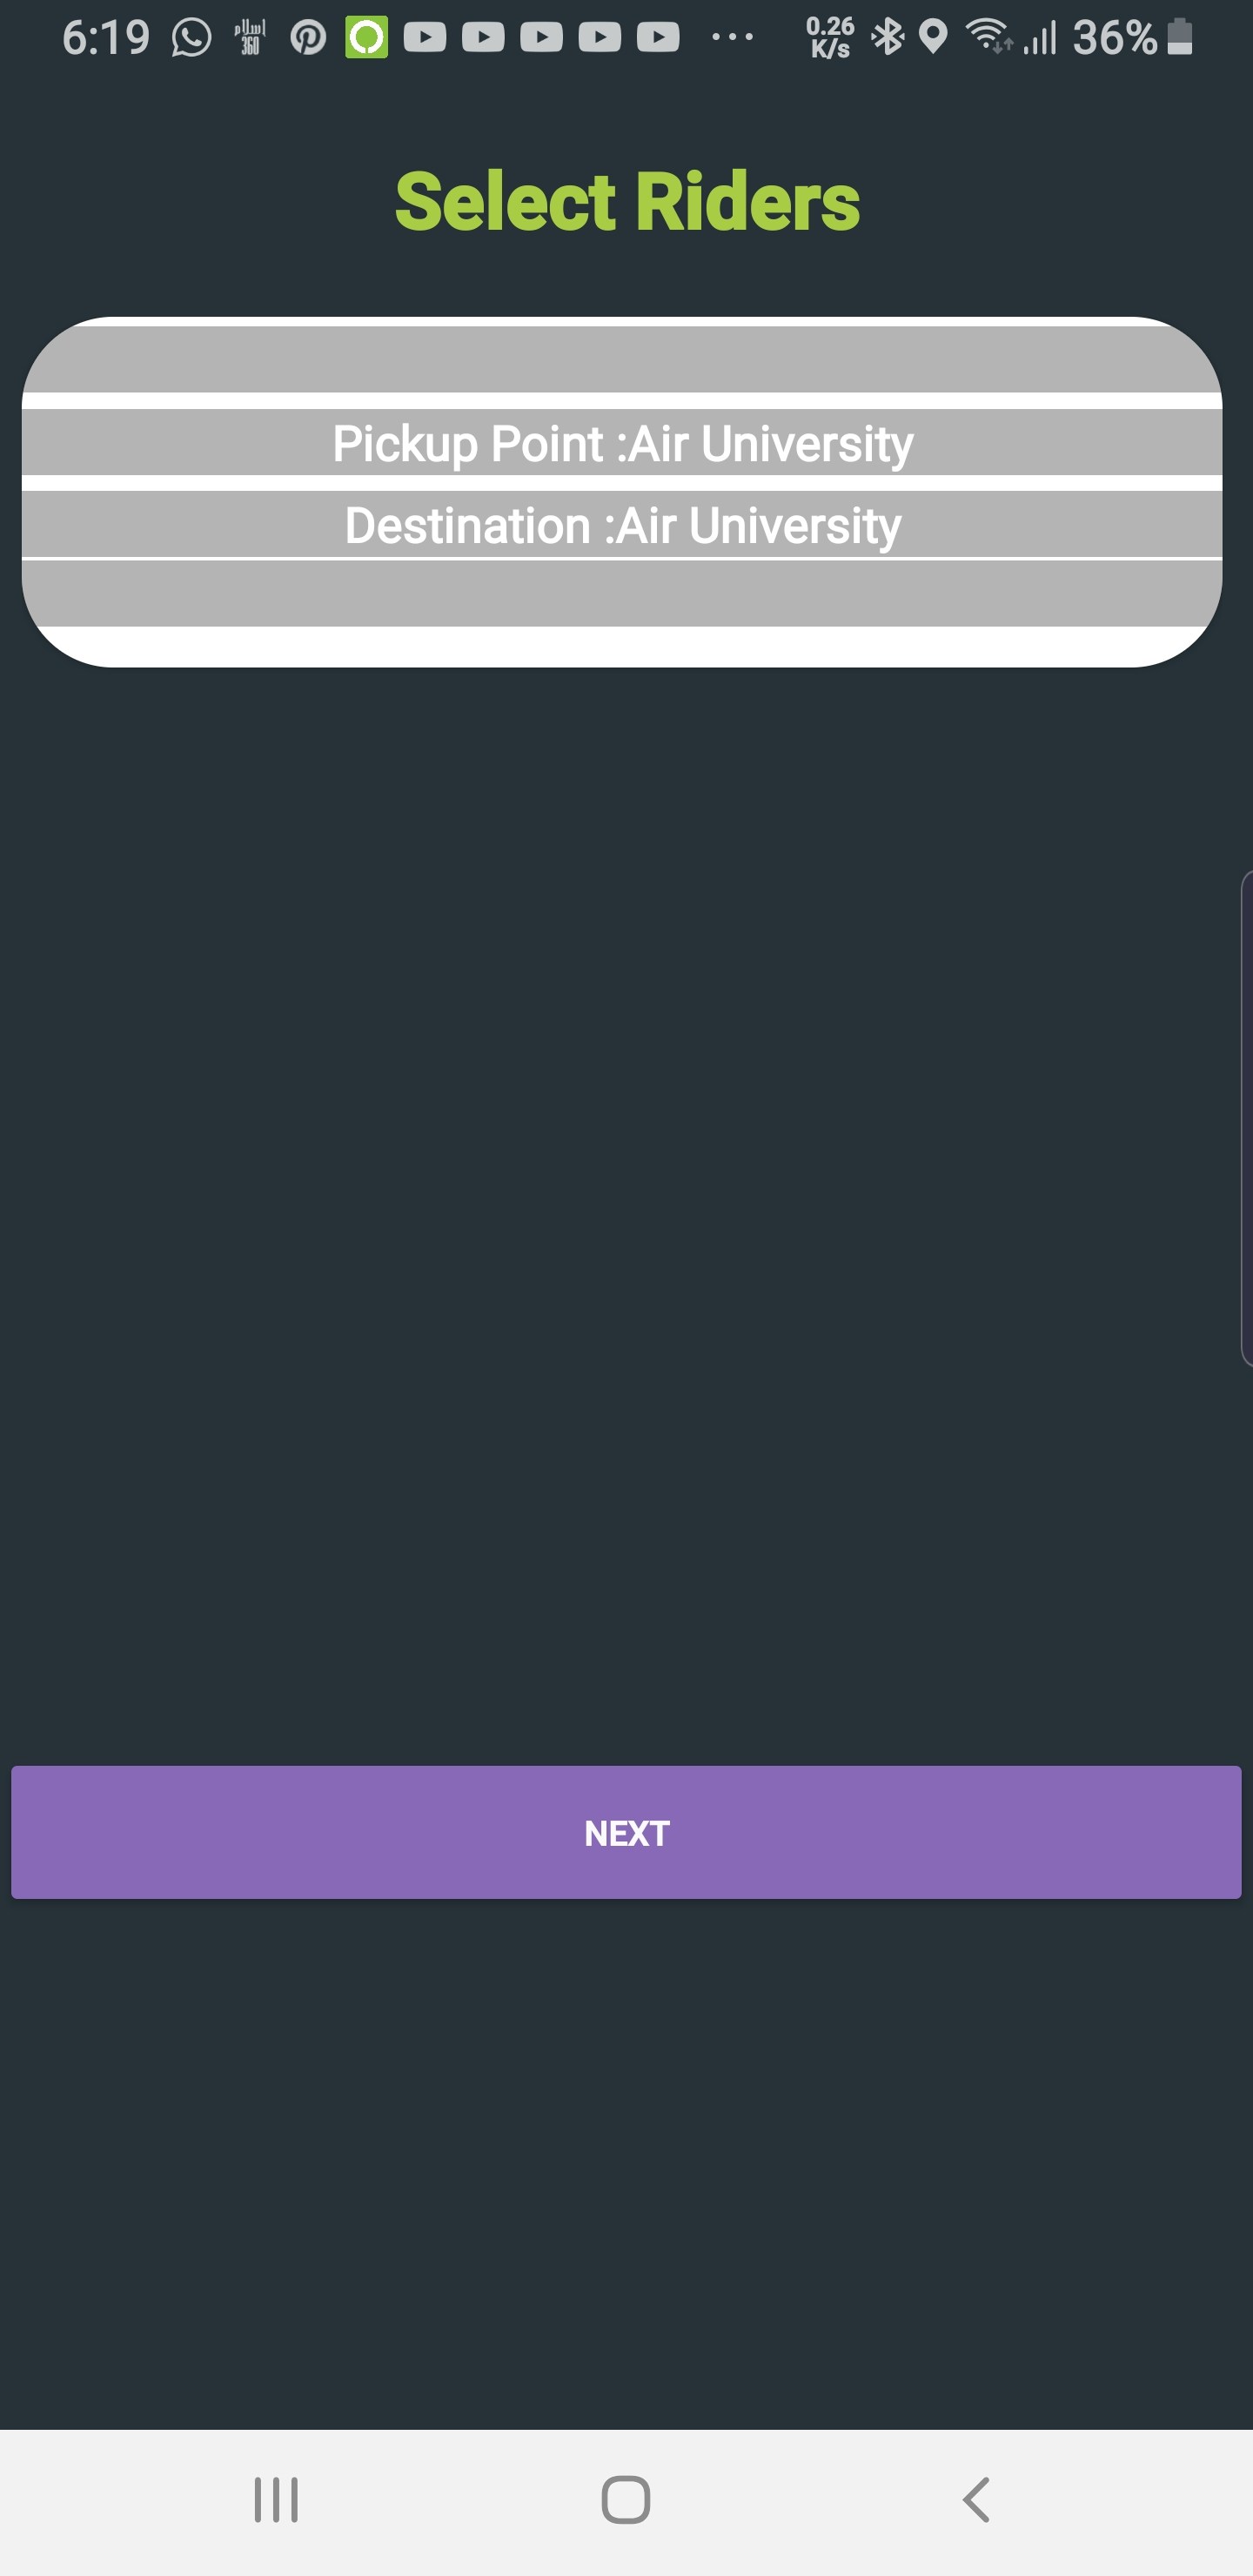
\includegraphics[width = 1.75in]{S12}}\hfill 
\subfloat[Popup Selection Confirmation Screen]{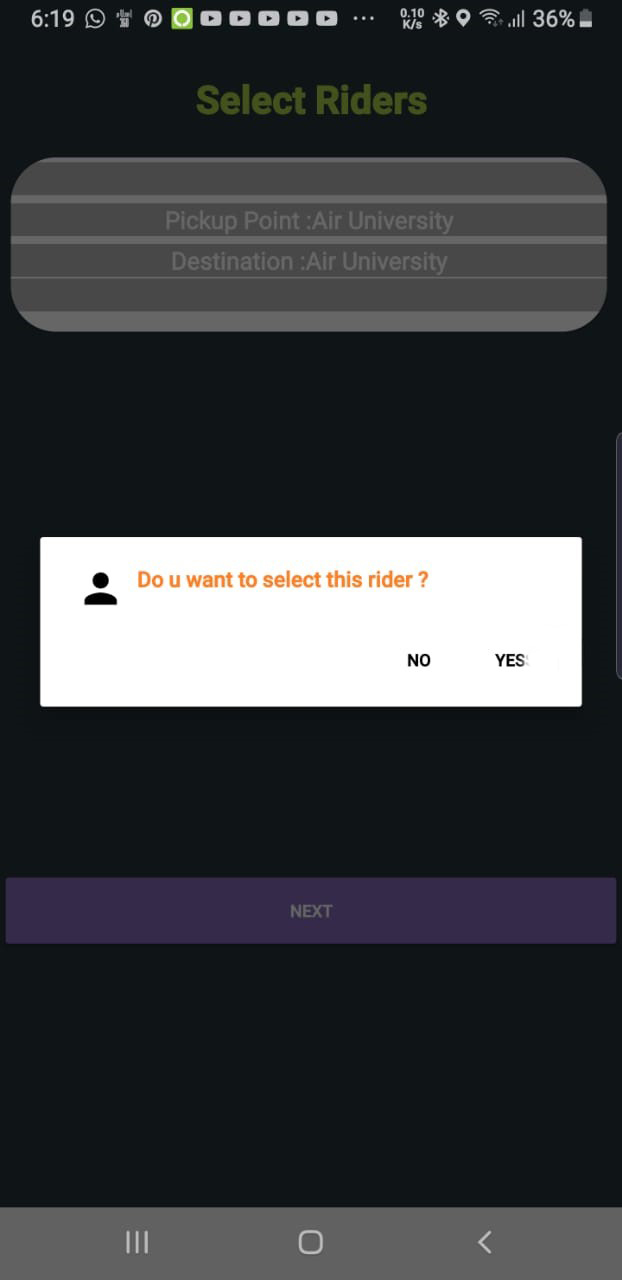
\includegraphics[width = 1.75in]{S13}}\hfill
\subfloat[Driver Summary Screen]{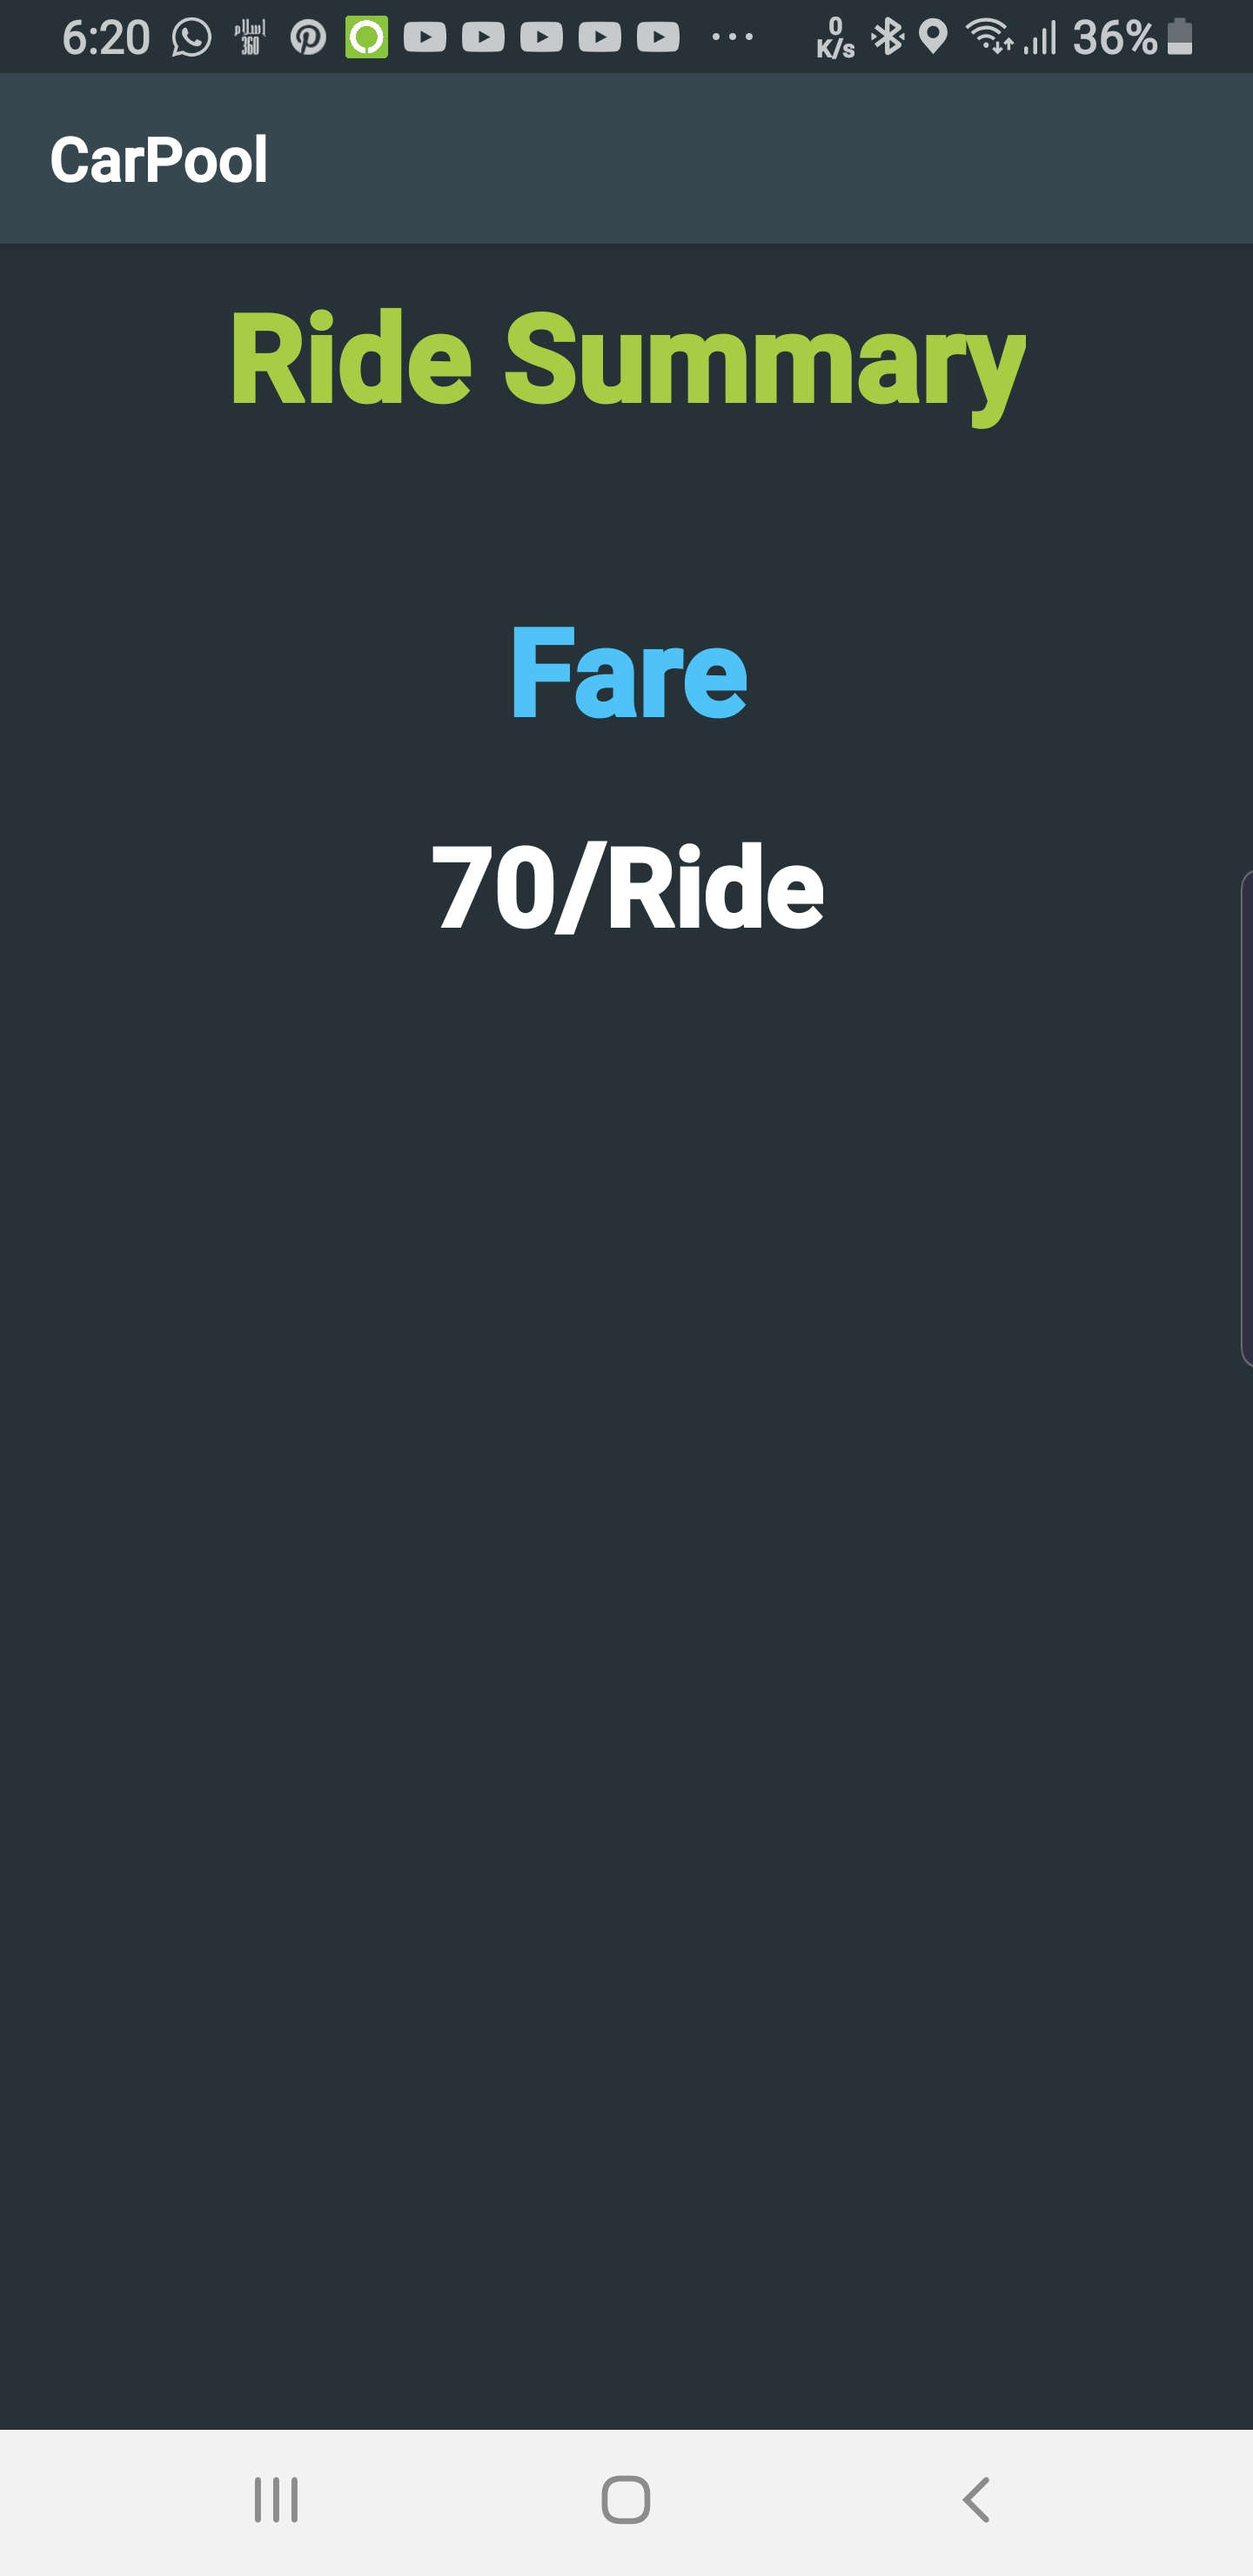
\includegraphics[width = 1.75in]{S16}}
\end{figure}